% !TeX TS-program = lualatex
% use lualatex because of academicons

%\documentclass[11pt,a4paper,onecolumn]{article}
\documentclass[11pt,a4paper,onecolumn,openany]{book}

% -- begin Packages

\usepackage[utf8]{inputenc}
\usepackage[T1]{fontenc}
\usepackage{amsmath}
\usepackage{amsfonts}
\usepackage{amssymb}
\usepackage{graphicx}
\usepackage[left=2.00cm, right=2.00cm, top=2.00cm, bottom=2.00cm]{geometry}

% Package for Style customization in single-sided documents
\usepackage{fancyhdr}


%\usepackage{lipsum}
\usepackage{wrapfig}
%\usepackage{fontawesome}
\usepackage{fontawesome5}
\usepackage{academicons}
\usepackage{enumitem}
\usepackage{worldflags}

%\usepackage[brazil,english]{babel}
\usepackage[brazil]{babel}

% --
% for including individual full refecenre in text
% --
\usepackage[square,numbers]{natbib}
\usepackage{bibentry}
\nobibliography*
% --

\usepackage[colorlinks=true, 
linkcolor=blue, 
urlcolor=blue,
citecolor=blue
]{hyperref}


\frenchspacing % Better looking spacings after periods
%\pagestyle{empty}           % No pagenumbers/headers/footers

% The command above will ensure that if two files are encountered with the same basename 
% but different extensions (for example image.eps, image.pdf, image.jpeg and image.png), 
% then the .eps version will be used first, .pdf version will be used second, .jpeg will be used
% third and finnaly the .png will be used in the absence of other versions
\DeclareGraphicsExtensions{.eps,.pdf,.jpeg,.png,.jpg}

% -- end Packages

% -- begin Macros

\newcommand{\FundingEntry}[9]{
	% agency, language, title, language, title, id, grant name, amount, period
	\noindent #1, Título (#2): \textit{#3}, Título (#4): \textit{#5}, ID: #6, Modalidade: #7, R\$ #8, #9.}

\newcommand{\ThesisEntry}[9]{
	% type (MSc or PhD), ID flag worldflag, title, ID flag worldflag, title, student, institution, year conclusion, my participation
	\def\tempa{#1}%
	\def\tempb{#2}%
	\def\tempc{#3}%
	\def\tempd{#4}%
	\def\tempe{#5}%
	\def\tempf{#6}%
	\def\tempg{#7}%
	\def\temph{#8}%
	\def\tempi{#9}%
	\ThesisEntrycont
}
\newcommand{\ThesisEntrycont}[1]{
	% doi number
	\noindent \textbf{[\tempa]}
	Título (\tempb): \textit{\tempc}, Título (\tempd): \textit{\tempe}, 
	Autor(a): \tempf, 
	\textsl{\tempg} (\temph). [\textsf{#1}].  \sloppy{\texttt{\textbf{doi:}}~\href{https://doi.org/\tempi}{\texttt{\tempi}}}}

\newcommand{\Student}[5]{
	% #1 level (MSc or PhD), #2 main or co supervisor, #3 name, since #4, #5 institution
	\noindent \textbf{[#1]} Estudante: #2, \textbf{#3} \dotfill 
	\parbox{0.17\textwidth}{\hfill desde~#4} \\
	\noindent\textsl{#5}}

% -- end Macros

\makeindex

\begin{document}

% -- begin title page
	
\begin{titlepage}
	\begin{center}
		\vspace*{3cm}

		\LARGE
		\textbf{Memorial das atividades científicas}

		\vspace{2.5cm}
		\large
		\textbf{Vanderlei C. Oliveira Jr.}

		\hspace{.45\textwidth}
		\begin{minipage}{.5\textwidth}
			\vspace{3.0cm}
			\normalsize
			Memorial das atividades científicas submetido à Comissão de Promoção de
			Pesquisadores e Tecnologistas (CPPT) do Observatório Nacional (ON) para
			ingresso na classe \textbf{Titular III} do cargo de \textbf{Pesquisador},  
			carreira de \textbf{Pesquisa em Ciência e Tecnologia}, de acordo com 
			a Lei no 8.691, que dispõe sobre o Plano de Carreiras para a área de 
			Ciência e Tecnologia da Administração Federal Direta, das Autarquias e 
			das Fundações Federais.
		\end{minipage}%
		\vspace*{\fill}

		\vspace{0.8cm}
			
		\small
		Observatório Nacional\\
		Coordenação de Geofísica \\
		Julho, 2022

	\end{center}
\end{titlepage}

% -- end title page

% -- begin summary
\fancyhf{}
\tableofcontents
\fancyhf{}
% -- end summary

% set customized page style with package fancyhdr
\pagestyle{fancy}
\fancyhf{}
\rhead{}
\lhead{Capítulo \thechapter: \chaptername}
\rfoot{\thepage}

\section*{Informações}

\begin{wrapfigure}{r}{-0.10\textwidth} 
	\centering
	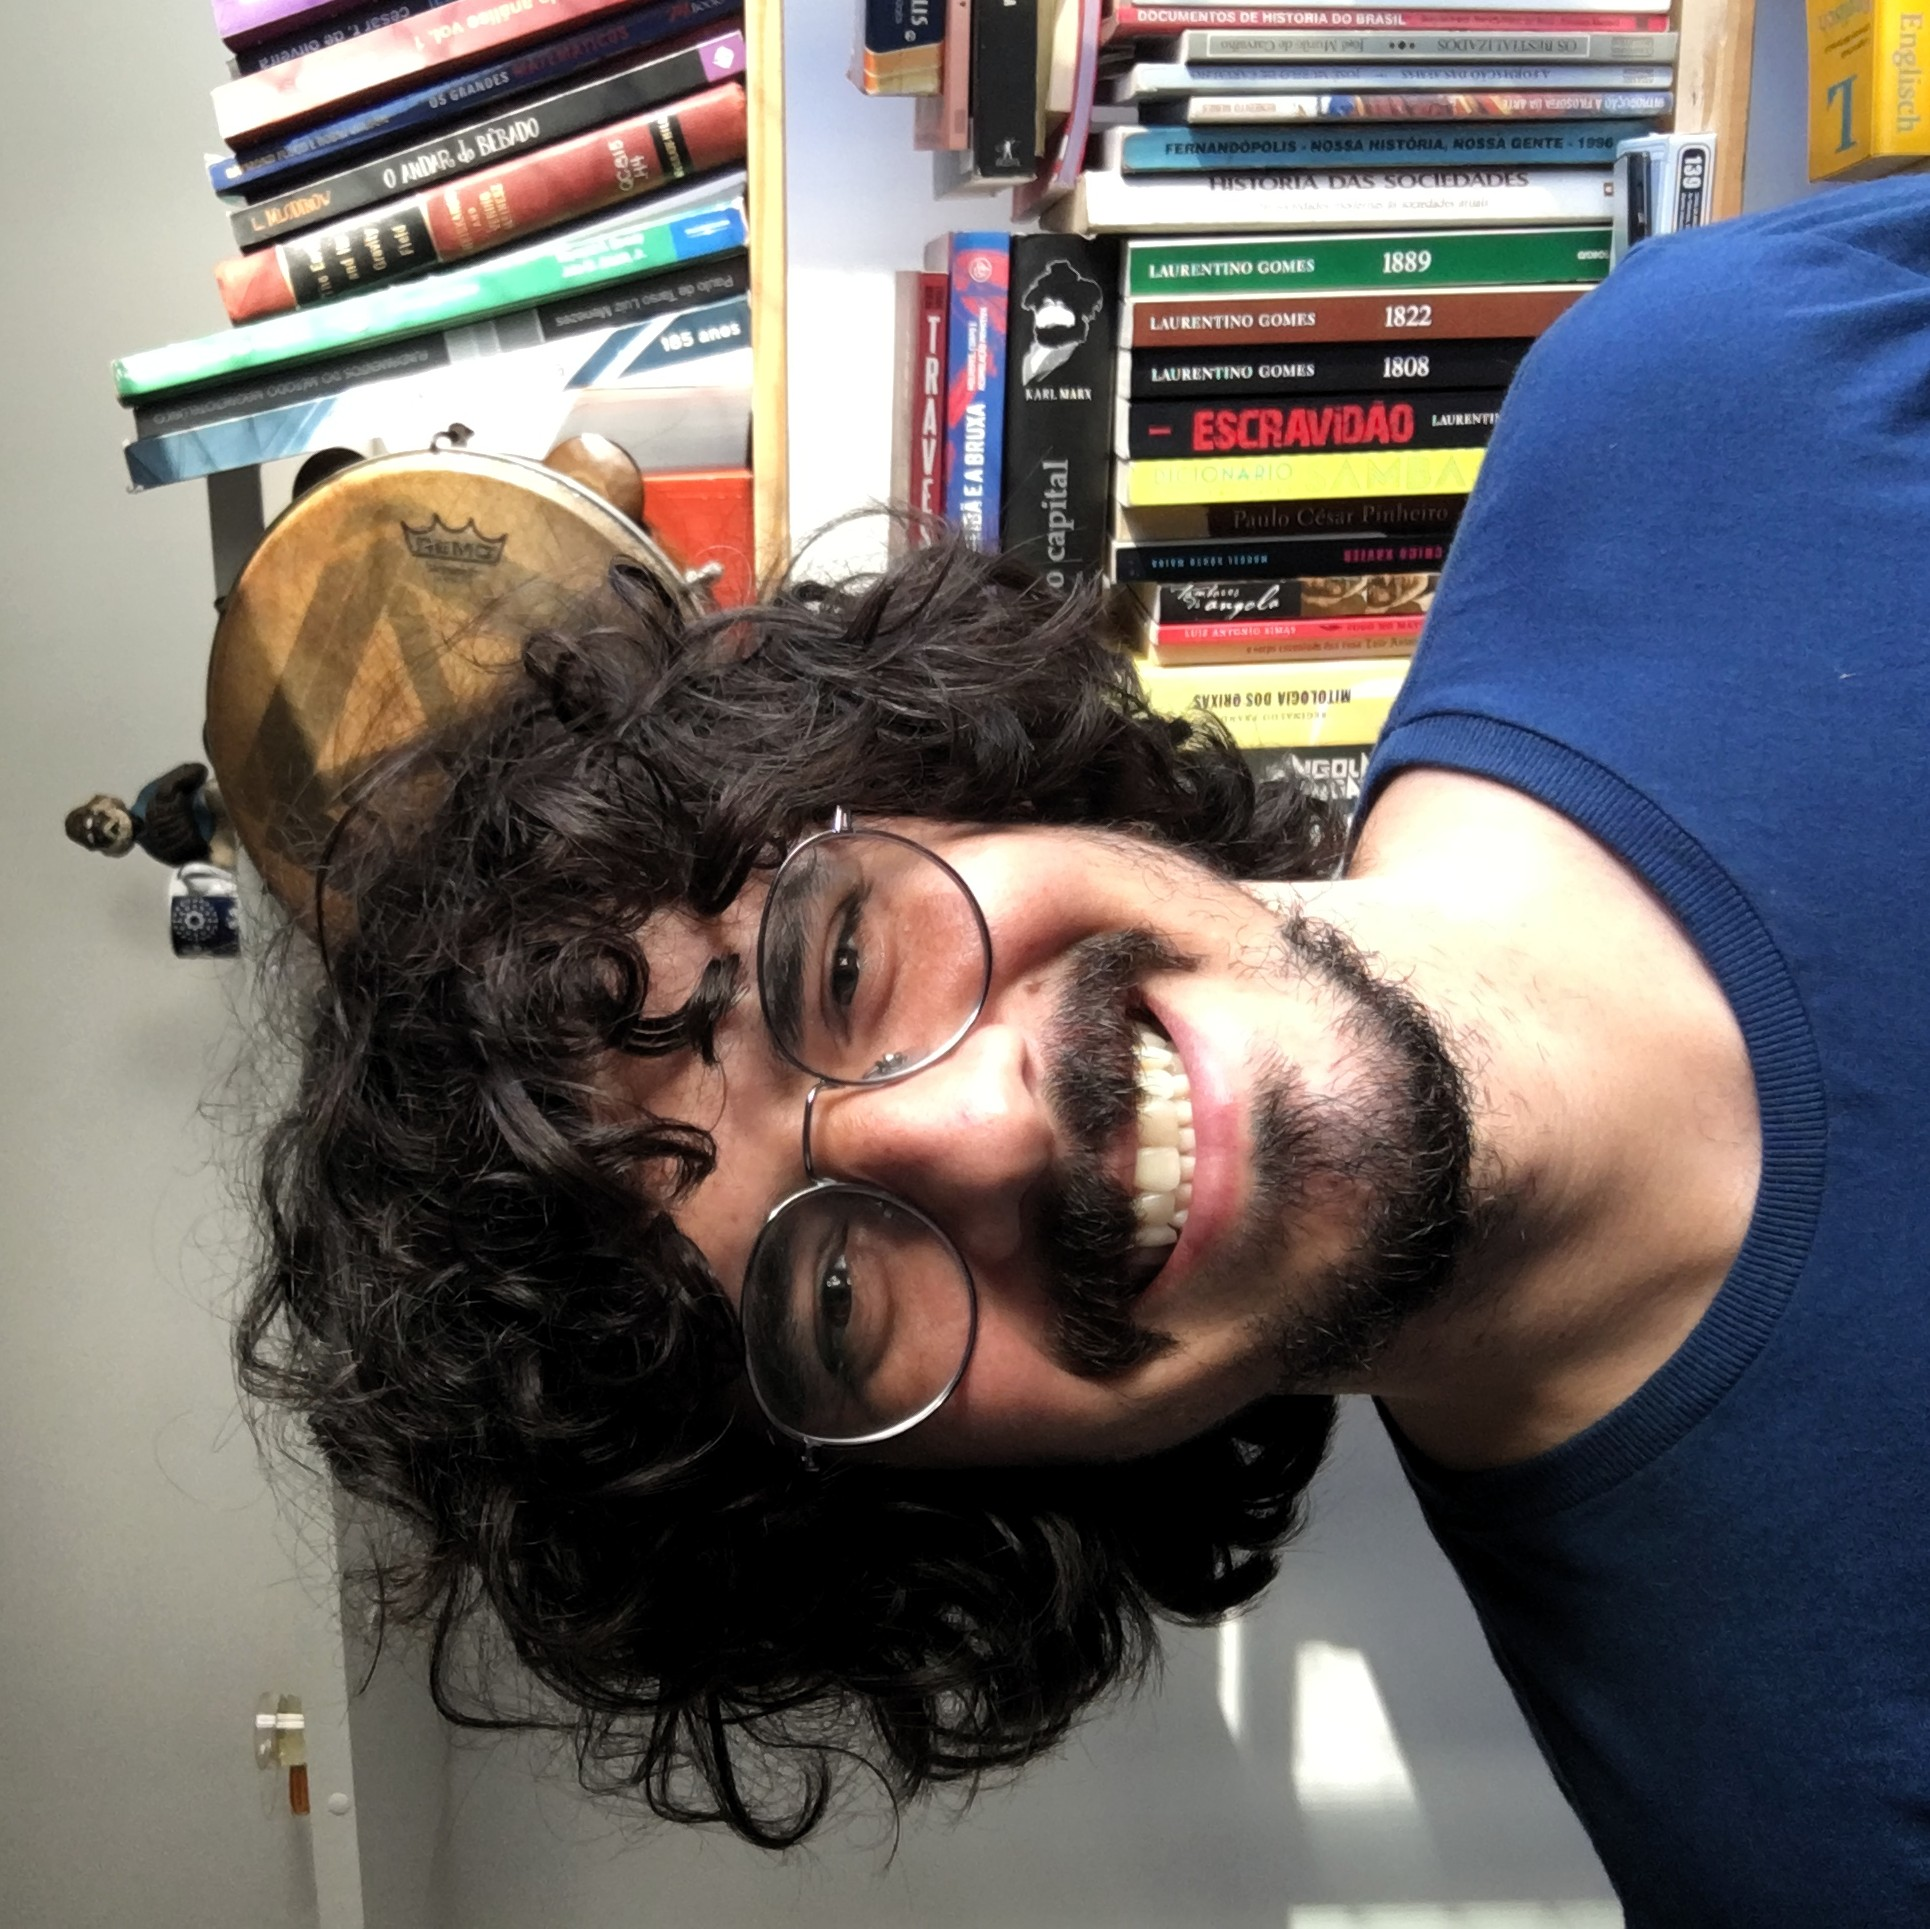
\includegraphics[width=0.35\textwidth]{foto}
\end{wrapfigure}

{\Large \faUser} \textbf{Vanderlei C. Oliveira Jr.}\\
{\Large \faInstitution} \href{https://www.on.br/index.php/pt-br/}{Observatório Nacional}\\
{\Large \faEnvelope} \href{mailto:vanderlei@on.br}{vanderlei@on.br}\\
{\Large \faEnvelopeO} \href{mailto:vandscoelho@gmail.com}{vandscoelho@gmail.com}\\
{\Large \faGroup} \href{http://www.pinga-lab.org/people/oliveira-jr.html}{pinga-lab.org/people/oliveira-jr}\\
{\Large \faInfoCircle} \href{http://lattes.cnpq.br/4332841435949533}{lattes.cnpq.br/4332841435949533}\\
{\Large \faInfoCircle} \href{http://orcid.org/0000-0002-6338-4086}{orcid.org/0000-0002-6338-4086}\\


%%% Education
%%% ------------------------------------------------------------
\section*{Formação}

\subsection*{Doutorado em Geof{\'i}sica}

%\faGraduationCap \quad \textbf{Doutorado em Geof{\'i}sica}\\
\faHourglassStart \quad Dez/2010 -- Jan/2013\\
\faInstitution \quad \href{http://www.on.br/index.php/pt-br/}{Observat{\'o}rio Nacional}\\
\faExternalLink \quad  \href{http://www.pinga-lab.org/thesis/oliveira-jr-phd.html}{Processamento e invers\~{a}o de dados de campos potenciais: Novas abordagens}\\
\textbf{Orientadora:} Dra. Valéria C. F. Barbosa \\
\textbf{Descrição:} Desenvolvi duas metodologias para o 
processamento e interpretação de dados gravimétricos e magnetométricos. A primeira é
a \textit{Camada Equivalente Polinomial} (\textit{Polynomial Equivalent Layer}), que 
é uma metodologia computacionalmente eficiente para processar grandes volumes de dados 
via técnica da camada equivalente. A segunda é uma metodologia para estimar a geometria 
de corpos 3D isolados via inversão não-linear de dados de gradiometria da gravidade.\\


\subsection*{Mestrado em Geof{\'i}sica}

%\faGraduationCap \quad \textbf{Mestrado em Geof{\'i}sica}\\
\faHourglassStart \quad Mar/2009 -- Nov/2010\\
\faInstitution \quad \href{http://www.on.br/index.php/pt-br/}{Observat{\'o}rio Nacional}\\
\faExternalLink \quad  \href{http://www.pinga-lab.org/thesis/oliveira-jr-msc.html}{Invers{\~a}o gravim{\'e}trica radial por camadas para a reconstru{\c c}{\~a}o de corpos geol{\'o}gicos 3D}\\
\textbf{Orientadora:} Dra. Valéria C. F. Barbosa \\
\textbf{Descrição:} Desenvolvi uma metodologia para
estimar a geometria de um corpo geol{\'o}gico 3D via invers{\~a}o n{\~a}o-linear 
de dados gravimétricos.\\


\subsection*{Bacharelado em Geof{\'i}sica}

%\faGraduationCap \quad \textbf{Bacharelado em Geof{\'i}sica}\\
\faHourglassStart \quad Mar/2004 -- Dez/2008\\
\faInstitution \quad \href{https://www.iag.usp.br/}{Instituto de Astronomia, Geof{\'i}sica e Ci{\^e}ncias Atmosf{\'e}ricas da Universidade de S{\~a}o Paulo}\\
\faExternalLink \quad Modelagem gravim{\'e}trica 3D da borda norte da Bacia do Paran{\'a}\\
\textbf{Orientadora:} Dra. Yára R. Marangoni \\
\textbf{Descrição:} Apliquei uma metodologia para estimar a geometria do 
embasamento e da Moho a partir da inversão não-linear de dados gravimétricos 
sobre a borda norte da Bacia do Paraná.


%\NewPart{Research interests}{}
%
%{\begin{itemize}
%
%	\item{\textbf{Equivalent layer technique:} computationally efficient methods 
%	for processing and interpreting large potential field data sets.}
%	
%	\item{\textbf{Inversion of gravity and/or magnetic data:} methods to invert gravity 
%	and/or magnetic data for the purpose of estimating the position and shape of geological
%	bodies.}
%	
%	\item{\textbf{Magnetization of geological bodies:} methods for estimating the
%	magnetization direction of geological bodies by using land and airborne magnetic data.}
%	
%	\item{\textbf{Magnetization of rock samples:} methods for estimating the magnetization
%	distribution within rock samples by using scanning magnetic microscopy data.}
%	
%	\item{\textbf{Magnetic modeling of geological bodies:} methods for computing the
%	demagnetizing field within geological bodies having high susceptibility.}
%	
%	\item{\textbf{Regional characterization of gravity field:} computationally efficient
%	methods for representing the regional gravity field by combining different data sets.}
%	
%	\item{\textbf{Regional characterization of the crustal magnetic field:} computationally
%	efficient methods for representing the crustal field by combining different data sets.}
%
%\end{itemize}}

%\vspace{2cm}
\renewcommand{\chaptername}{Capítulo}
\chapter{Resumo das atividades científicas}
\renewcommand{\chaptername}{Resumo das atividades científicas}
\label{cap:resumo-atividades}

Neste capítulo, apresento um resumo das atividades científicas -- que incluem pesquisa, 
ensino, orientação e atividades institucionais -- desenvolvidas por mim ao longo da minha
carreira. É importante ressaltar que, no presente capítulo,
as atividades são apresentadas sem a devida contextualização, de forma meramente 
descritiva. Uma apresentação mais detalhada sobre as atividades de pesquisa, ensino e
orientação é feita no Capítulo \ref{cap:detalhe-atividades}.


\section{Pesquisa}
\label{sec:pesquisa}

Desde quando iniciei a minha carreira científica realizo pesquisa básica e aplicada em
Geofísica, com ênfase na área de métodos potenciais, sobre os seguintes temas:

\begin{itemize}
	
	\item[\parbox{0.03\textwidth}{\vspace{-0.1\baselineskip}\faSearch}] 
	{\textbf{Teoria do potencial aplicada:} investigações teóricas sobre transformações de campos gravitacionais e magnéticos produzidos por fontes 3D;}
	
	\item[\parbox{0.03\textwidth}{\vspace{-0.1\baselineskip}\faSearch}] 
	{\textbf{Métodos numéricos:} desenvolvimento de métodos computacionalmente eficientes para o processamento e interpretação de grandes volumes de dados;}
	
	\item[\parbox{0.03\textwidth}{\vspace{-0.1\baselineskip}\faSearch}] 
	{\textbf{Inversão de dados gravimétricos e magnéticos:} desenvolvimento de métodos para estimar a posição e a forma de fontes 3D;}
	
	\item[\parbox{0.03\textwidth}{\vspace{-0.1\baselineskip}\faSearch}] 
	{\textbf{Magnetização de corpos geológicos:} desenvolvimento de métodos para estimar a direção de magnetização de fontes 3D a partir de dados magnéticos provenientes de levantamentos aéreos e terrestres;}
	
	\item[\parbox{0.03\textwidth}{\vspace{-0.1\baselineskip}\faSearch}] 
	{\textbf{Magnetização de amostras de rocha:} desenvolvimento de métodos para estimar a direção de magnetização de amostras de rocha a partir de dados de microscopia magnética por varredura;}
	
	\item[\parbox{0.03\textwidth}{\vspace{-0.1\baselineskip}\faSearch}] 
	{\textbf{Modelagem gravimétrica e magnética:} desenvolvimento de métodos e implementação computacional de algoritmos para calcular os campos gravitacional e magnético produzidos por fontes 3D e o cálculo do campo desmagnetizante no interior de corpos geológicos com alta suscetibilidade;}
	
	\item[\parbox{0.03\textwidth}{\vspace{-0.1\baselineskip}\faSearch}] 
	{\textbf{Caracterização regional do campo de gravidade:} desenvolvimento de métodos para a representação do campo de gravidade regional a partir da combinação de diferentes conjuntos de dados gravimétricos;}
	
	\item[\parbox{0.03\textwidth}{\vspace{-0.1\baselineskip}\faSearch}] 
	{\textbf{Caracterização regional do campo magnético crustal:} desenvolvimento de métodos para a representação do campo magnético crustal a partir da combinação de diferentes conjuntos de dados magnéticos.}
	
\end{itemize}

\section{Observatório Nacional, Brasil}

\subsection*{Vínculo institucional}

\begin{itemize}
	\item[\parbox{0.03\textwidth}{\vspace{-0.3\baselineskip}\faClipboardList}]
	{Pesquisador Titular II \dotfill \parbox{0.11\textwidth}{\hfill 2021--hoje}} 
	\item[\parbox{0.03\textwidth}{\vspace{-0.3\baselineskip}\faClipboardCheck}]
	{Pesquisador Titular I \dotfill \parbox{0.11\textwidth}{\hfill 2020--2021}}
	\item[\parbox{0.03\textwidth}{\vspace{-0.3\baselineskip}\faClipboardCheck}]
	{Pesquisador Associado III \dotfill \parbox{0.11\textwidth}{\hfill 2018--2020}}
	\item[\parbox{0.03\textwidth}{\vspace{-0.3\baselineskip}\faClipboardCheck}]
	{Pesquisador Associado II \dotfill \parbox{0.11\textwidth}{\hfill 2017--2018}}
	\item[\parbox{0.03\textwidth}{\vspace{-0.3\baselineskip}\faClipboardCheck}]
	{Pesquisador Associado I \dotfill \parbox{0.11\textwidth}{\hfill 2016--2017}}
	\item[\parbox{0.03\textwidth}{\vspace{-0.3\baselineskip}\faClipboardCheck}]
	{Pesquisador Adjunto III \dotfill \parbox{0.11\textwidth}{\hfill 2015--2016}}
	\item[\parbox{0.03\textwidth}{\vspace{-0.3\baselineskip}\faClipboardCheck}]
	{Pesquisador Adjunto II \dotfill \parbox{0.11\textwidth}{\hfill 2014--2015}}
	\item[\parbox{0.03\textwidth}{\vspace{-0.3\baselineskip}\faClipboardCheck}]
	{Pesquisador Adjunto I \dotfill \parbox{0.11\textwidth}{\hfill 2013--2014}}
	
\end{itemize}

\subsection*{Atividades institucionais}

\begin{itemize}
	
	\item[\parbox{0.03\textwidth}{\vspace{-0.1\baselineskip}\faUserCheck}]
	{Membro da comissão de pós-graduação em Geofísica \dotfill \parbox{0.11\textwidth}{\hfill 2020--hoje} \newline \textit{Portaria ON 20/2020 - 5/08/2020}} 
	
	\item[\parbox{0.03\textwidth}{\vspace{-0.1\baselineskip}\faUserCheck}]
	{Coordenador do programa de pós-graduação em Geofísica \dotfill \parbox{0.11\textwidth}{\hfill 2017--2018} \newline \textit{Portaria ON 22/2017 - 29/05/2017}}
	
	\item[\parbox{0.03\textwidth}{\vspace{-0.1\baselineskip}\faUserCheck}]
	{Membro da comissão de dados abertos \dotfill \parbox{0.11\textwidth}{\hfill 2017--2019} \newline \textit{Portaria ON 7/2017 - 8/03/2017}}

	\item[\parbox{0.03\textwidth}{\vspace{-0.1\baselineskip}\faUserCheck}]
	{Membro da comissão de pós-graduação em Geofísica \dotfill \parbox{0.11\textwidth}{\hfill 2015--2017} \newline \textit{Portaria ON 7/2015 - 18/03/2015}}

	\item[\parbox{0.03\textwidth}{\vspace{-0.1\baselineskip}\faUserCheck}]
	{Membro do corpo docente permanente do programa de pós-graduação em Geofísica \dotfill \parbox{0.11\textwidth}{\hfill 2014--hoje} \newline \textit{Portaria ON 7/2015 - 18/03/2015}}

	\item[\parbox{0.03\textwidth}{\vspace{-0.1\baselineskip}\faUserCheck}]
	{Membro da comissão do Programa de Capacitação Institucional (PCI) \dotfill \parbox{0.11\textwidth}{\hfill 2013--2014} \newline \textit{Portaria ON 44/2013 - 15/10/2013}}
	
\end{itemize}


\subsection*{Atividades de ensino e orientação}


Ingressei como membro do corpo docente permanente do Programa de Pós-Graduação em
Geofísica do Observatório Nacional (PPGG-ON) em 2014. Desde então, 
concluí a orientação de \textbf{4 (quatro)} teses de doutorado e 
\textbf{4 (quatro)} dissertações de mestrado como \textbf{orientador principal},
bem como \textbf{2 (duas)} teses de doutorado e \textbf{2 (duas)} dissertações de
mestrado como \textbf{co-orientador} sobre diversos temas relacionados às minhas
linhas de pesquisa. Atualmente, oriento \textbf{2 (duas)} dissertações de mestrado
como orientador principal e \textbf{2 (duas)} teses de doutorado como co-orientador
no PPGG-ON. 
Além disso, atuo como docente responsável desde 2014 por \textbf{2 (duas)} disciplinas 
no PPGG-ON.

\clearpage

\section{Institut Universitaire Européen de la Meer (IUEM), França}


\subsection*{Vínculo institucional}


\begin{itemize}
	
	\item[\parbox{0.03\textwidth}{\vspace{-0.3\baselineskip}\faClipboardCheck}]
	{Pesquisador visitante \dotfill \parbox{0.11\textwidth}{\hfill 2018--2019}} 
	
\end{itemize}

\subsection*{Atividades de ensino e orientação}

Ao longo dos anos de 2018 e 2019, atuei como pesquisador visitante no 
\href{https://www-iuem.univ-brest.fr/lgo/le-labo/}{\textit{Laboratoire Géosciences Océan}}, 
do
\href{https://www-iuem.univ-brest.fr/}{\textit{Institut Universitaire Européen de la Meer}},
França.
Naquele período, trabalhei juntamente com a 
\href{https://www-iuem.univ-brest.fr/lgo/equipe/maia-marcia-do-carmo/}{Dra. Marcia Maia} 
e o 
\href{https://www-iuem.univ-brest.fr/lgo/equipe/tarits-pascal/}{Dr. Pascal Tarits} 
na interpretação de dados magnéticos na Zona de Falhas Transformantes de São
Paulo (ZFTSP), próximo ao arquipélago de São Pedro e São Paulo, e
\textbf{co-orientei um trabalho de mestrado}.



\section{Liverpool University, Reino Unido}


\subsection*{Vínculo institucional}


\begin{itemize}
	
	\item[\parbox{0.03\textwidth}{\vspace{-0.3\baselineskip}\faClipboardList}]
	{Honorary PGR Supervisor \dotfill \parbox{0.11\textwidth}{\hfill 2021--2024}} 
	
\end{itemize}

\subsection*{Atividades de ensino e orientação}

Desde 2021, atuo como \textbf{co-orientador de uma tese de doutorado} no 
âmbito do projeto de pesquisa \textit{``Improving estimates of Antarctic geothermal heat flow from magnetic data''}. Este projeto está sendo desenvolvido no departamento de
\href{https://www.liverpool.ac.uk/earth-ocean-and-ecological-sciences/}{\textit{Earth, Ocean and Ecological Sciences}} da 
\href{https://www.liverpool.ac.uk/}{\textit{Liverpoool University}}, Reino Unido, em
conjunto com o 
\href{https://www.liverpool.ac.uk/environmental-sciences/staff/leonardo-uieda/}{Dr. Leonardo Uieda} (orientador principal e coordenador do projeto) e o
\href{https://www.liverpool.ac.uk/environmental-sciences/staff/richard-holme/}{Dr. Richard Holme}.


\section{Compilação das principais atividades}


Abaixo apresento uma lista com as minhas principais atividades científicas:

\begin{itemize}
	\item[\parbox{0.03\textwidth}{\vspace{-0.1\baselineskip}\faHandHoldingWater}]
	\textbf{2 (duas)} orientações de mestrado em andamento como orientador principal;
	\item[\parbox{0.03\textwidth}{\vspace{-0.1\baselineskip}\faHandsHelping}]
	\textbf{2 (duas)} orientações de doutorado em andamento como coorientador;
	\item[\parbox{0.03\textwidth}{\vspace{-0.1\baselineskip}\faHandshake}]
	\textbf{1 (uma)} supervisão de pós doutorado em andamento;
	\item[\parbox{0.03\textwidth}{\vspace{-0.1\baselineskip}\faGraduationCap}]
	Conclusão de \textbf{4 (quatro)} orientações de mestrado como orientador principal e outras \textbf{3 (três)} como co-orientador;
	\item[\parbox{0.03\textwidth}{\vspace{-0.1\baselineskip}\faGraduationCap}]
	Conclusão de \textbf{4 (quatro)} orientações de doutorado como orientador principal e outras \textbf{2 (duas)} como co-orientador;
	\item[\parbox{0.025\textwidth}{\vspace{-0.1\baselineskip}\faGlasses}]
	Conclusão de \textbf{2 (duas)} supervisões de pós doutorado;
	\item[\parbox{0.03\textwidth}{\vspace{-0.1\baselineskip}\faPencil*}]
	Publicação de \textbf{20 (vinte)} artigos em periódicos de circulação internacional;
	\item[\parbox{0.03\textwidth}{\vspace{-0.1\baselineskip}\faPeopleCarry}]
	Desenvolvimento de cooperações nacionais e internacionais;
	\item[\parbox{0.03\textwidth}{\vspace{-0.1\baselineskip}\aiIDEASRePEc}] 
	Coordenação de \textbf{3 (três)} projetos financiados pelo CNPq
	(\textit{Universal} e \textit{Bolsas PQ});
	\item[\parbox{0.03\textwidth}{\vspace{-0.1\baselineskip}\aiIDEASRePEc}]
	Coordenação de \textbf{2 (dois)} projetos financiados pela FAPERJ
	(\textit{Auxílio Instalação} e \textit{JCNE});
	\item[\parbox{0.03\textwidth}{\vspace{-0.1\baselineskip}\faBomb}]
	Coordenação do Programa de Pós-Graduação em Geofísica do ON.

\end{itemize}

\renewcommand{\chaptername}{Capítulo}
\chapter{Apresentação detalhada das atividades científicas}
\renewcommand{\chaptername}{Apresentação detalhada das atividades científicas}
\label{cap:detalhe-atividades}

Neste capítulo, apresento as atividades de pesquisa, ensino e orientação que venho
realizando ao longo da minha carreira de forma contextualizada e mais detalhada 
do que aquela do Capítulo \ref{cap:resumo-atividades}. 
A primeira seção é dedicada exclusivamente às minhas atividades de ensino.
As seções seguintes descrevem meus projetos de pesquisa, bem como a produção científica,
formação de recursos humanos e captação de recursos financeiros associada aos mesmos.


\section{Atividades de ensino}
\label{sec:ensino}

Desde quando ingressei no corpo docente permanente do Programa de Pós-Graduação em 
Geofísica do Observatório Nacional (PPGG-ON), atuo como docente responsável pelas
duas disciplinas listadas abaixo e mantenho o conteúdo das mesmas disponibilizado 
livremente em repositórios do GitHub.

\begin{itemize}
	\item[\parbox{0.03\textwidth}{\vspace{-0.1\baselineskip}\faChalkboardTeacher}]
	{\textbf{Métodos potenciais}\\ 
	\href{https://github.com/birocoles/Disciplina-metodos-potenciais}
	{\texttt{https://github.com/birocoles/Disciplina-metodos-potenciais}}};
	
	\item[\parbox{0.03\textwidth}{\vspace{-0.1\baselineskip}\faChalkboardTeacher}]
	{\textbf{Métodos computacionais aplicados à Geofísica}\newline
	\href{https://github.com/birocoles/Disciplina-metodos-computacionais}
	{\texttt{https://github.com/birocoles/Disciplina-metodos-computacionais}}};
\end{itemize}

%\subsection*{Contextualização e considerações pessoais sobre a relação docência $\times$ pesquisa}

As duas disciplinas pelas quais sou responsável no PPGG-ON estão diretamente relacionadas
às minhas linhas de pesquisa (Seção \ref{sec:pesquisa}). Por isso, minhas atividades de
docência e pesquisa se retroalimentam constantemente. Se por um lado dar 
aula é uma oportunidade para revisitar conceitos fundamentais na realização da minha
pesquisa, por outro a minha pesquisa é fundamental para que eu possa incluir tópicos 
mais avançados nas disciplinas. 

Outro aspecto importante da atividade como docente é a criação constante de material 
didático. Além do conteúdo disponibilizado nos repositórios mencionados acima, comecei a
organizar em 2020 as minhas notas de aula da disciplina de Métodos Potenciais com o intuito
de gerar um material mais robusto. Embora o projeto ainda esteja muito no começo,
o objetivo é escrever um livro. Outro projeto que também comecei recentemente é o
desenvolvimento de um pacote com metodologias venho desenvolvendo com meu grupo de pesquisa
desde que ingressei no ON. Este projeto também está em estágio inicial.


%\subsection*{Considerações pessoais sobre o ensino de Geofísica}
%
%Depois da orientação de estudantes, considero a docência como a atividade mais difícil 
%da minha carreira. 
%Acho que dar aulas sobre geofísica na pós-graduação no Brasil é um grande desafio, uma vez
%que é uma área (i) muito mais 
%recente do que outras áreas como engenharia, física e geologia\footnote{CORDANI, UMBERTO G. et al. Ensino de Geociências na universidade. Estudos Avançados. 2018, v. 32, n. 94, pp. 309-330. ISSN 1806-9592. doi:  \href{https://doi.org/10.1590/s0103-40142018.3294.0020}{10.1590/s0103-40142018.3294.0020}.},
%por exemplo, e (ii) muito interdisciplinar.
%Na minha opinião, estes dois fatores dificultam o estabelecimento de um consenso sobre quais
%são os requisitos mínimos que devem compor a formação básica de um geofísico nos cursos de 
%graduação e o que deve ser considerado como formação avançada nos cursos de pós-graduação
%em geofísica brasileiros. Considero que estes fatores também explicam o número relativamente
%baixo de pesquisadores e professores universitários com graduação em geofísica atuantes em
%departamentos de graduação e pós-graduação em geofísica. 
%
%Os primeiros cursos de graduação em Geofísica do Brasil foram criados na 
%\href{https://www.iag.usp.br/hist%C3%B3ria-do-iag}{Universidade de São Paulo (USP)}, 
%em 1984; na \href{http://www.cpgg.ufba.br/gr-geof/}{Universidade Federal da Bahia (UFBA)};
%em 1992; e na 
%\href{http://www.ig.ufpa.br/index.php/historico}{Universidade Federal do Pará (UFPA)}, 
%em 2003. 
%Na cidade do Rio de Janeiro, sede do Observatório Nacional, o primeiro e único curso de
%graduação em Geofísica foi criado na
%\href{http://www.geofisica.uff.br/node/1}{Universidade Federal Fluminense (UFF)}, em 2004.
%Atualmente, outras 4 universidades brasileiras além destas listas acima oferecem cursos de
%graduação em Geofísica. São elas: 
%\href{https://sigaa.ufrn.br/sigaa/public/departamento/portal.jsf?id=4894}{Universidade Federal do Rio Grande do Norte (UFRN)}, 
%\href{http://igd.unb.br/index.php?option=com_content&view=article&id=14&Itemid=132}{Universidade de Brasilia (UnB)}, 
%\href{https://cursos.unipampa.edu.br/cursos/geofisica/o-curso/}{Universidade Federal do Pampa (UNIPAMPA)} e 
%\href{https://sigaa.ufopa.edu.br/sigaa/public/curso/portal.jsf?id=14&lc=pt_BR&nivel=G}{Universidade Federal do Oeste do Pará (UFOPA)}.
%Já os primeiros cursos de pós-graduação em geofísica antecedem os primeiros cursos de
%graduação nessa área. Segundo consta na página da área de Geociências da CAPES\footnote{\href{https://www.gov.br/capes/pt-br/acesso-a-informacao/acoes-e-programas/avaliacao/sobre-a-avaliacao/areas-avaliacao/sobre-as-areas-de-avaliacao/colegio-de-ciencias-exatas-tecnologicas-e-multidisciplinar/ciencias-exatas-e-da-terra/geociencias}{Documento de área mais recente, de 2019}}, 
%há 5 programas de pós-graduação em geofísica no Brasil atualmente.
%O PPGG-ON, assim como acredito que aconteça nos outros programas da área de geofísica,
%recebe estudantes formados em diferentes cursos de graduação e considero que
%isso cria o seguinte paradigma: ao mesmo tempo que é necessário fornecer conhecimentos
%avançados em relação aos cursos de graduação em geofísica, também é necessário fornecer
%conhecimentos básicos sobre geofísica aos estudantes que vêm de outras áreas.

%No PPGG-ON, do total de 12 docentes
%permanentes, sou o único com graduação em geofísica. No programa de pós-graduação do
%IAG-USP, 4 dos 15 docentes permentes têm graduação em geofísica. NA UFBA, também há apenas
%um docente permanente com graduação em geofísica no programa de pós-graduação em geofísica.
%
%Para mim, a principal consequência do baixo número de pessoas com graduação em geofísica
%atuando no ensino de geofísica no Brasil é o viés específico em detrimento a formação mais
%ampla que deveria nortear os cursos de graduação em geofísica.
%
%
%Acredito que é muito mais difícil
%para um(a) pesquisador(a) ou professor(a) universitário(a) dar aulas de geofísica, sobretudo
%nos cursos de graduação, se este(a) 

%e considero que há pelo menos três motivos para isso.
%
%O primeiro deles é que lidamos com pessoas, que em geral são muito mais complicadas 
%do que estudar o planeta Terra.
%
%O segundo motivo é que, na minha opinião, não há um consenso sobre quais são
%os requisitos mínimos que devem compor a formação básico de um geofísico nos cursos de 
%graduação e, muito menos, nos curso de pós-graduação brasileiros.
%Acredito que, somente a partir da definição de um perfil básico 
%
%clareza sobre quais são os quesitos
%mínimos que devem constar na formação 
%
%mínimos para que  é o perfil 
%que se espera de um 
%deve ser considerado
%um curso de ``pós-graduação" em geofísica no Brasil.
%
%O \href{https://www.gov.br/observatorio/pt-br/assuntos/programas-academicos/pos-graduacao-em-geofisica/o-programa}{PPGG-ON} 
%foi criado em 1981, como parte do Programa de Pós-Graduação em Astronomia
%do Observatório Nacional, e tornou-se independente entre os anos de 1998 e 1999.
%Em 2007, o PPGG-ON passou por uma grande reestruturação, que praticamente definiu a
%sua estrutura atual.
%
%É importante ressaltar que, naquela época, havia pouquíssimos geofísicos no Brasil.
%Os primeiros cursos de graduação em Geofísica do Brasil foram criados na 
%\href{https://www.iag.usp.br/hist%C3%B3ria-do-iag}{Universidade de São Paulo (USP)}, 
%em 1984; na \href{http://www.cpgg.ufba.br/gr-geof/}{Universidade Federal da Bahia (UFBA)};
%na \href{http://www.ig.ufpa.br/index.php/historico}{Universidade Federal do Pará (UFPA)}, 
%em 2003; na 
%\href{https://sigaa.ufrn.br/sigaa/public/departamento/portal.jsf?id=4894}{Universidade Federal do Rio Grande do Norte (UFRN)}, 
%entre os anos de 2007 e 2008; e na
%\href{http://igd.unb.br/index.php?option=com_content&view=article&id=14&Itemid=132}{Universidade de Brasilia (UnB)}, em 2008.
%Na cidade do Rio de Janeiro, sede do Observatório Nacional, o primeiro e único curso de
%graduação em Geofísica foi criado na
%\href{http://www.geofisica.uff.br/node/1}{Universidade Federal Fluminense (UFF)}, em 2004.

\clearpage

%%%%%%%%%%% begin Projeto da Daiana
\section{Estimativa da direção da magnetização total de corpos 3D aproximadamente esféricos}
\label{sec:projeto-Daiana}

\noindent{\parbox{0.03\textwidth}{\vspace{-0.2\baselineskip} \faCalendarCheck[regular]}}
2014 -- 2017
\vspace{0.3\baselineskip}\\
\noindent\parbox{0.03\textwidth}{\vspace{-0.2\baselineskip}\faUniversity}
\href{https://www.gov.br/observatorio/pt-br}{\textsl{Observatório Nacional}}
\parbox{0.03\textwidth}{\vspace{-0.2\baselineskip} \hfill \worldflag[width=3mm,stretch=1]{BR}} 


\subsection*{Objetivos}

Desenvolver uma metodologia computacionalmente eficiente para estimar a direção da 
magnetização total de corpos aproximadamente esféricos a partir da inversão da 
anomalia de campo total. Os recursos financeiros recebidos pelas agências de fomento 
foram utilizados para comprar material de consumo, prover recursos computacionais e 
custear a divulgação dos resultados em congressos internacionais.

\subsection*{Orientações concluídas}

\begin{enumerate}
	
	\item\ThesisEntry{Mestrado}{portugu{\^e}s}{Estimativa do vetor de magnetiza\c{c}\~{a}o total de corpos aproximadamente esf\'{e}ricos}{ingl{\^e}s}{Estimating the total magnetization vector of approximately spherical bodies}{Daiana P. Sales}{Observat\'{o}rio Nacional, Brasil}{2014}{10.6084/m9.figshare.20334867.v1}{orientador principal}
	
\end{enumerate}

\subsection*{Financiamentos}

\begin{enumerate}
	
	\item\FundingEntry{\href{https://cnpq.br/pagina-inicial}{Conselho Nacional de Desenvolvimento Cient\'{i}fico e Tecnol\'{o}gico (CNPq)}}{português}{Estimativa da dire\c{c}\~{a}o da magnetiza\c{c}\~{a}o total de corpos 3D aproximadamente esf\'{e}ricos}{inglês}{Estimation of the total magnetization direction of approximately 3D spherical bodies}{445752/2014-9}{MCTI/CNPQ/Universal 14/2014}{20~000.00}{Nov/2014 -- Nov/2017}
	
	\item\FundingEntry{\href{https://www.faperj.br/}{Funda\c{c}\~{a}o Carlos Chagas Filho de Amparo \`{a} Pesquisa do Estado do Rio de Janeiro (FAPERJ)}}{português}{Infraestrutura computacional para a estima\c{c}\~{a}o da magnetiza\c{c}\~{a}o de corpos 3D aproximadamente dipolares}{inglês}{Computational infrastructure for estimating the magnetization direction of approximately dipolar bodies}{E-26/111.152/2014}{INST - Aux{\' i}lio Instala{\c c}{\~ a}o - 2013/2 }{10~000.00}{Jun/2014 -- Mar/2016}
	
\end{enumerate}

\subsection*{Resumos em anais de congressos}

\begin{enumerate}
	\item \bibentry{iugg_2015a}
\end{enumerate}

\subsection*{Artigos em periódicos indexados}

\begin{enumerate}
	\item \bibentry{oliveirajr_etal_2015}
\end{enumerate}

\subsection*{Contextualização e considerações pessoais}

Este projeto começou logo que entrei no ON, em 2013, e foi desenvolvido ao longo do
mestrado da então estudante \href{https://lattes.cnpq.br/7941053288321760}{Daiana de Paula Sales}, que trabalha na CPRM até hoje.
Comecei como coorientador da dissertação e, em 2014, tornei-me o orientador principal.
Considero que a ideia desenvolvida ao longo do projeto é relativamente simples,
mas foi extremamente importante para a minha carreira. Foi a partir dela que pude conduzir a 
minha primeira orientação na pós-graduação e tive meus primeiros projetos de pesquisa
aprovados por agências de fomento. Até hoje penso que orientar 
é a atividade mais difícil na carreira de um(a) pesquisador(a).

%%%%%%%%%%% end Projeto da Daiana

%%%%%%%%%%% begin Projeto do André - mestrado
\section{Desenvolvimento de métodos para processamento e interpretação de dados de microscopia magnética}
\label{sec:projeto-Andre}

\noindent{\parbox{0.03\textwidth}{\vspace{-0.2\baselineskip}\faCalendar*[regular]}} 2014 -- presente
\vspace{0.3\baselineskip}\\
\noindent\parbox{0.03\textwidth}{\vspace{-0.2\baselineskip}\faUniversity}
\href{https://www.gov.br/observatorio/pt-br}{\textsl{Observatório Nacional}}
\parbox{0.03\textwidth}{\vspace{-0.2\baselineskip} \hfill \worldflag[width=3mm,stretch=1]{BR}} \\
\noindent\parbox{0.03\textwidth}{\vspace{-0.2\baselineskip}\faUniversity}
\href{https://www.puc-rio.br/index.html}{\textsl{PUC-Rio}}
\parbox{0.03\textwidth}{\vspace{-0.2\baselineskip} \hfill \worldflag[width=3mm,stretch=1]{BR}} \\
\noindent\parbox{0.03\textwidth}{\vspace{-0.2\baselineskip}\faUniversity}
\href{https://www.uerj.br/}{\textsl{Universidade do Estado do Rio de Janeiro (UERJ)}}
\parbox{0.03\textwidth}{\vspace{-0.2\baselineskip} \hfill \worldflag[width=3mm,stretch=1]{BR}} \\
\noindent\parbox{0.03\textwidth}{\vspace{-0.2\baselineskip}\faUniversity}
\href{https://www5.usp.br/}{\textsl{Universidade de São Paulo (USP)}}
\parbox{0.03\textwidth}{\vspace{-0.2\baselineskip} \hfill \worldflag[width=3mm,stretch=1]{BR}} \\
\noindent\parbox{0.03\textwidth}{\vspace{-0.2\baselineskip}\faUniversity}
\href{https://www.unb.br/}{\textsl{Universidade de Brasília (UnB)}}
\parbox{0.03\textwidth}{\vspace{-0.2\baselineskip} \hfill \worldflag[width=3mm,stretch=1]{BR}}


\subsection*{Objetivos}

Desenvolver métodos de processamento e interpretação de dados de microscopia magnética 
de varredura aplicada à caracterização de amostras de rocha para estudos paleomagnéticos 
e de magnetismo de rochas. Este projeto é desenvolvido em colaboração com 
pesquisadores do 
\href{https://www.fgel.uerj.br/site/departamentos/depto-de-geologia-aplicada/dgap-quadro-de-pessoal/}{Departamento de Geologia Aplicada da UERJ} e do
\href{https://www.fis.puc-rio.br/instrumentacao-e-medidas-magneticas/}{Laboratório de Instrumentação e Medidas Magnéticas da PUC-Rio}.

\subsection*{Orientações concluídas}

\begin{enumerate}
	
	\item\ThesisEntry{Mestrado}{portugu{\^e}s}{Invers\~{a}o magn\'{e}tica 3D para estimar a distribui\c{c}\~{a}o de magnetiza\c{c}\~{a}o de uma amostra de rocha}{ingl{\^e}s}{3D Magnetic inversion to estimate the magnetization distribution of a rectangular rock sample}{Andr\'{e} L. A. Reis}{Observat\'{o}rio Nacional, Brasil}{2016}{10.6084/m9.figshare.20335209.v1}{orientador principal}
	
\end{enumerate}

\subsection*{Resumos em anais de congressos}

\begin{enumerate}
	\item \bibentry{latinmag_2017}
	\item \bibentry{agu_fallmeeting_2016a}
	\item \bibentry{iugg_2015b}
\end{enumerate}

\subsection*{Artigos em periódicos indexados}

\begin{enumerate}
	\item \bibentry{araujo_etal2019_materials}
	\item \bibentry{araujo_etal2019_sensors}
	\item \bibentry{reis_etal2016}
	
\end{enumerate}

\subsection*{Contextualização e considerações pessoais}
\label{subsec:projeto-Andre-consideracoes}

No final de 2013, o Dr. \href{https://lattes.cnpq.br/3934334115083849}{Ricardo Trindade} (IAG-USP) arranjou uma reunião na
PUC-Rio com o objetivo de discutir eventuais colaborações na área de microscopia
magnética. Essa colaboração envolvia o grupo do Dr Ricardo, especializado em
paleomagnetismo e magnetismo de rochas, o grupo do Dr \href{https://lattes.cnpq.br/8840926029509231}{Antônio Carlos Bruno}
(PUC-Rio), especializado em instrumentação científica na área de magnetismo,
o grupo do Dr \href{https://eapsweb.mit.edu/people/limaea}{Eduardo Lima Andrade} (MIT, USA), que estava no Brasil, trabalha com paleomagnetismo,
magnetismo de rochas e também a parte de instrumentação, e o grupo da Dra. Valéria
Barbosa (ON), que trabalha com inversão de dados.
Para a reunião, o Ricardo levou o então recém-doutor (orientado por ele)
\href{https://lattes.cnpq.br/9806242954314478}{Elder Yokoyama}, e eu fui junto com a 
Val. Também estavam presentes o chefe
do laboratório de instrumentação onde aconteceu a reunião na PUC-Rio, o Dr.
Antônio Carlos Bruno, e o Dr. Eduardo Lima Andrade.
Foi naquela reunião que surgiu a ideia de aplicar métodos de processamento e
interpretação de dados magnéticos provenientes de levantamentos terrestres e 
aéreos a dados de microscopia magnética produzidos por amostras de rocha,
medidos em laboratório.
Ainda em 2013, o Dr Elder Yokoyama iniciou um estágio de pós-doutorado no ON,
sob minha supervisão, para trabalhar com microscopia magnética.

Em 2014, comecei a orientar outra dissertação de mestrado. 
Eu fui o orientador principal e o Dr Elder Yokoyama foi o coorientador. 
A ideia era desenvolver métodos para o processamento e interpretação 
de dados de microscopia magnética de varredura. Ao longo deste projeto, o Dr. Elder
coordenou a confecção das amostras de rocha no IAG-USP, o grupo do Dr. Antônio Carlos Bruno
ficou responsável pelas medidas no microscópio magnético desenvolvido por eles na PUC-Rio 
e eu coordenei o desenvolvimento dos métodos de processamento e interpretação dos dados
no ON.

Ainda que o projeto seja basicamente a aplicação e técnicas comumente usadas na 
magnetometria para interpretar dados produzidos por amostras de rocha, ele representou 
uma ligeira mudança de área na minha carreira. Tão importante quanto concluir a 
orientação de outra dissertação de mestrado e estabelecer minha primeira colaboração foi 
publicar, ao longo deste projeto, meus primeiros trabalhos sem a participação da 
minha amiga e principal parceira de trabalho, a Valéria. Isso foi fundamental para 
eu poder seguir minha carreira dentro do ON. Obviamente voltei a 
trabalhar com ela em projetos posteriores, mas dessa vez por opção e não por necessidade.

Em 2014, o Dr. Elder deixou o estágio de pós doutorado no ON para assumiu o cargo de
professor no 
\href{http://www.pesquisar.unb.br/professor/elder-yokoyama}{Instituto de Geociências da Universidade de Brasília (UnB)}. 
Eu e ele seguimos a orientação da dissertação do então estudante de mestrado e hoje
Dr. \href{https://lattes.cnpq.br/1075610796165589}{André Luis Albuquerque dos Reis},
\href{https://www.fgel.uerj.br/site/departamentos/depto-de-geologia-aplicada/dgap-quadro-de-pessoal/}{professor do Departamento de Geologia Aplicada} 
na Faculdade de Geologia da Universidade do
Estado do Rio de Janeiro (UERJ). A dissertação foi defendida em 2016.
Após este trabalho, o André iniciou o doutorado no ON, sob minha orientação e
coorientação da Valéria, e ficou à frente da colaboração com a PUC-Rio. 
Já na PUC-Rio, a colaboração passou a ser coordenada pelo Dr. \href{https://lattes.cnpq.br/0190128964748843}{Jefferson Ferraz Damasceno
Felix Araújo}, que concluiu o doutorado na PUC-Rio em 2013, sob a orientação do 
Dr. Antônio Carlos Bruno. Atualmente o Jefferson é o professor responsável pelo 
\href{https://www.fis.puc-rio.br/instrumentacao-e-medidas-magneticas/}{Laboratório de Instrumentação e Medidas Magnéticas da PUC-Rio}.
Mantemos esta colaboração até os dias de hoje.
%%%%%%%%%%% end Projeto do André - mestrado

\clearpage

%%%%%%%%%%% begin Projeto do Diego - mestrado
\section{Modelagem magnética de corpos com alta suscetibilidade} 
\label{sec:projeto-Diego}

\noindent{\parbox{0.03\textwidth}{\vspace{-0.2\baselineskip}\faCalendarCheck[regular]}} 2014 -- 2017
\vspace{0.3\baselineskip}\\
\noindent\parbox{0.03\textwidth}{\vspace{-0.2\baselineskip}\faUniversity} \href{https://www.gov.br/observatorio/pt-br}{\textsl{Observatório Nacional}}
\parbox{0.03\textwidth}{\vspace{-0.2\baselineskip} \hfill \worldflag[width=3mm,stretch=1]{BR}}

\subsection*{Objetivos}

É comum considerar que corpos geológicos são magnetizados uniformemente quando são 
submetidos a um campo magnético uniforme. Esta premissa falha quando os corpos possuem 
alta suscetibilidade magnética devido a um fenômeno chamado auto-desmagnetização 
(self-demagnetization). Negligenciar este efeito para corpos com alta suscetibilidade 
pode levar a resultados espúrios obtidos a partir da interpretação de anomalias 
magnéticas. 
Ao longo deste projeto, foi desenvolvido um método para a modelagem e interpretação 
de dados magnéticos produzidos por corpos geológicos que possuem altos valores de 
suscetibilidade e/ou anisotropia de suscetibilidade e que podem ser aproximados por 
elipsoides. Também foi desenvolvido um novo critério numérico para definir o limite 
no valor da suscetibilidade magnética isotrópica a partir do qual o efeito de 
auto-desmagnetização deve ser levado em consideração.

\subsection*{Orientações concluídas}

\begin{enumerate}
	
	\item\ThesisEntry{Mestrado}{portugu{\^e}s}{Modelagem magn\'{e}tica 3D de corpos elipsoidais}{ingl{\^e}s}{3D Magnetic modeling of elipsoidal bodies}{Diego Takahashi}{Observat\'{o}rio Nacional, Brasil}{2017}{10.6084/m9.figshare.20335221.v1}{orientador principal}
	
\end{enumerate}

\subsection*{Resumos em anais de congressos}

\begin{enumerate}
	\item \bibentry{sbgf_2016_elipsoid}
\end{enumerate}

\subsection*{Artigos em periódicos indexados}

\begin{enumerate}
	\item \bibentry{takahashi_oliveirajr2017}
	
\end{enumerate}

\subsection*{Contextualização e considerações pessoais}
\label{subsec:proeto-diego-consideracoes}

Este projeto foi importante na consolidação da minha independência na carreira,
uma vez que ele foi desenvolvido ao longo do mestrado do então estudante de mestrado e
hoje Dr. \href{https://lattes.cnpq.br/4939493474727725}{Diego Takahashi} e eu fui o
único orientador.
Diego sempre mostrou mais interesse na parte numérica e na programação, por isso 
considerei que este tema era adequado para ele.
A dissertação desenvolvida pelo Diego foi classificada entre as 10 (dez) finalistas no 
\href{https://www.geolsoc.org.uk/Education-and-Careers/Grants/Earth-Model-Award}{\textit{Earth Model Award 2017}}, organizado pela empresa Halliburton-Landmark.
Após concluir seu mestrado, ele ingressou no doutorado em geofísica do ON, sob minha
orientação e coorientação da Valéria.
%%%%%%%%%%% end Projeto do Diego - mestrado

\clearpage

%%%%%%%%%%% begin Projeto da Marcela - mestrado
\section{Inversão de dados de campos potenciais para estimar a geometria de multiplas superfícies} 
\label{sec:projeto-Marcela}

\noindent{\parbox{0.03\textwidth}{\vspace{-0.2\baselineskip}\faCalendarCheck[regular]}} 2016 -- 2020
\vspace{0.3\baselineskip}\\
\noindent{\parbox{0.03\textwidth}{\vspace{-0.2\baselineskip}\faUniversity}} \href{https://www.gov.br/observatorio/pt-br}{\textsl{Observatório Nacional}}
\parbox{0.03\textwidth}{\vspace{-0.2\baselineskip} \hfill \worldflag[width=3mm,stretch=1]{BR}}

\subsection*{Objetivos}

Dados gravimétricos e magnetométricos são utilizados há muito tempo para investigar 
a estrutura crustal em estudos locais. A estratégia mais comum é aproximar a crosta por 
um conjunto de camadas justapostas com propriedade física constante ou dependente 
da profundidade. Os limites destas camadas são definidos por superfícies que geralmente 
representam camadas sedimentares, a batimetria, o relevo do embasamento e a Moho. 
Problemas inversos que visam estimar a geometria destas superfícies sofrem, geralmente, 
de uma severa falta de unicidade, sobretudo nas situações em que a geometria de duas 
ou mais superfícies devem ser estimadas simultaneamente. Ao longo deste projeto, 
foi desenvolvido um método para estimar a geometria do embasamento e da Moho sob  
uma margem continental passiva por meio da inversão não-linear de dados 
gravimétricos. Para contornar a ambiguidade inerente a este problema, um vínculo 
isostático foi desenvolvido para impor suavidade no stress litostático produzido pela 
crosta e manto superior sobre uma superfície plana com profundidade constante. 
O método se mostrou útil na interpretação de dados de satélite 
sobre uma margem vulcânica com pronunciado afinamento crustal no sul do Brasil. 
Outro aspecto relevante do projeto foi mostrar que a imposição de equilíbrio isostático 
não remove a ambiguidade do problema. De fato, mostrou-se que é possível obter modelos 
que ajustam os dados igualmente e com diferentes graus de equilíbrio isostático.


\subsection*{Orientações concluídas}

\begin{enumerate}
	
	\item\ThesisEntry{Mestrado}{portugu{\^e}s}{Invers{\~ a}o gravim{\' e}trica 2D com v{\' i}nculo isost{\' a}tico}{ingl{\^e}s}{2D gravity inversion with isostatic constraint}{B. Marcela S. Bastos}{Observat\'{o}rio Nacional, Brasil}{2018}{10.6084/m9.figshare.20335263.v1}{orientador principal}
	
	\item\ThesisEntry{Mestrado}{portugu{\^e}s}{Investiga\c{c}\~{a}o geof\'{i}sica do Alto do Cear\'{a} na margem equatorial brasileira -- Uma crosta continental ou uma crosta oce\^{a}nica?}{ingl{\^e}s}{Geophysical investigation of the Cear\'{a} Rise in the brazilian equatorial margin -- A continental crust or oceanic crust?}{Victor C. Pereira}{Observat\'{o}rio Nacional, Brasil}{2017}{10.6084/m9.figshare.20340885.v1}{coorientador}
	
\end{enumerate}

\subsection*{Artigos em periódicos indexados}

\begin{enumerate}
	\item \bibentry{bastos_oliveirajr2020}
\end{enumerate}

\subsection*{Contextualização e considerações pessoais}

Em 2014, a Valéria começou a orientar a dissertação de mestrado do
\href{https://lattes.cnpq.br/5615324764745474}{Victor do Couto Pereira}. Como o Victor
já tinha certa experiência na indústria, o trabalho teve um cunho mais aplicado a
interpretação geofísica/geológica do que ao desenvolvimento de um método numérico,
especialidade do nosso grupo. Eu fui coorientador da dissertação dele.
O Victor defendeu sua dissertação em março de 2017 e hoje é empresário na
área de geofísica.

\bigskip

\noindent A partir do trabalho do Victor, tive a ideia de desenvolver um método 2D para interpretar
dados gravimétricos sobre perfis ao longo de uma bacia sedimentar localizada na margem
brasileira. Certamente o fato de ter trabalhado na graduação com inversão de dados
gravimétricos para estimar o relevo do embasamento 
(Seção \ref{sec:apresentacao-consideracoes}) contribuiu para a elaboração dessa ideia.
O principal objetivo foi incluir informação a priori sobre o equilíbrio isostático
ao longo do perfil. Essa ideia foi desenvolvida durante o mestrado da 
\href{https://lattes.cnpq.br/8080347874698745}{Bárbara Marcela dos Santos Bastos},
que ingressou no mestrado em 2016 sob minha orientação. 
Marcela já era funcionária da Petrobrás naquela época e trabalha
lá até hoje. Nesse sentido, esse tema parecia ideal para ela.
%%%%%%%%%%% end Projeto da Marcela - mestrado

%%%%%%%%%%% begin Projeto guarda-chuva camada equivalente computacional
\section{Métodos computacionalmente eficientes para o processamento, modelagem e interpretação de dados de campos potenciais} \label{sec:projeto-guarda-chuva-fast}

\noindent{\parbox{0.03\textwidth}{\vspace{-0.2\baselineskip}\faCalendar*[regular]}} 2010 -- presente
\vspace{0.3\baselineskip}\\
\noindent\parbox{0.03\textwidth}{\vspace{-0.2\baselineskip}\faUniversity} \href{https://www.gov.br/observatorio/pt-br}{\textsl{Observatório Nacional}}
\parbox{0.03\textwidth}{\vspace{-0.2\baselineskip} \hfill \worldflag[width=3mm,stretch=1]{BR}} \\
\noindent\parbox{0.03\textwidth}{\vspace{-0.2\baselineskip}\faUniversity}
\href{https://www.unina.it/home}{\textsl{Università Degli Studi Di Napoli Federico II}}
\parbox{0.03\textwidth}{\vspace{-0.2\baselineskip} \hfill \worldflag[width=3mm,stretch=1]{IT}}

\subsection*{Objetivos}

Grandes volumes de dados gravimétricos e magnetométricos requerem a utilização de 
metodologias computacionalmente eficientes para a seu processamento e interpretação. 
Sob determinadas condições, os métodos numéricos utilizados para o processamento e 
interpretação de dados de campos potenciais envolvem sistemas lineares que podem 
ser resolvidos de forma eficiente, por meio de métodos iterativos. Em outras situações, 
estes sistemas são equivalentes à uma operação de convolução discreta. Esta operação, 
por sua vez, pode ser muito eficiente do ponto de vista computacional quando calculada 
usando a transformada rápida de Fourier. O presente projeto propõe o desenvolvimento 
de métodos computacionalmente eficientes para resolver problemas de processamento, 
modelagem e interpretação de dados de campos potenciais que podem ser resolvidos de 
forma iterativa e/ou formulados como uma convolução discreta. 

\subsection*{Orientações concluídas}

\begin{enumerate}
	
	\item\ThesisEntry{Doutorado}{portugu{\^e}s}{Camada  equivalente convolucional para processamento de dados potenciais}{ingl{\^e}s}{Convolutional equivalent layer for potential-field data processing}{Diego Takahashi}{Observat\'{o}rio Nacional, Brasil}{2021}{10.6084/m9.figshare.20335446.v1}{orientador principal}
	
	\item\ThesisEntry{Doutorado}{portugu{\^e}s}{Modelagem regional do campo de gravidade utilizando pontos de massa em coordenadas geod{\' e}sicas}{ingl{\^e}s}{Regional gravity modeling by using point masses in geodetic coordinates}{Kristoffer A. T. Hallam}{Observat\'{o}rio Nacional, Brasil}{2019}{10.6084/m9.figshare.20335266.v1}{orientador principal}
	
	\item\ThesisEntry{Doutorado}{portugu{\^e}s}{Otimiza\c{c}\~{a}o computacional do m\'{e}todo da camada equivalente}{ingl{\^e}s}{Computational optimization of the equivalent layer method}{Fillipe C. L. Siqueira}{Observat\'{o}rio Nacional, Brasil}{2016}{10.6084/m9.figshare.20340975.v1}{coorientador}
	
\end{enumerate}

\subsection*{Orientações em andamento}

\begin{enumerate}
	\item\Student{Doutorado}{Larissa S. Piauilino}{co-orientador}{Jul/2018}{Observat{\'o}rio Nacional, Brasil} 
\end{enumerate}

\subsection*{Resumos em anais de congressos}

\begin{enumerate}
	\item \bibentry{seg_2020_conv_eqlayer}
	\item \bibentry{seg_2020_fast_mag_eqlayer}
	\item \bibentry{sbgf_2019_gradgrav}
	\item \bibentry{seg_2019_gradgrav}
	\item \bibentry{eage_2017_fast_eqlayer}
	\item \bibentry{agu_fallmeeting_2016b}
\end{enumerate}

\subsection*{Artigos em periódicos indexados}

\begin{enumerate}
	\item \bibentry{takahashi_etal2022}
	\item \bibentry{takahashi_etal2020}
	\item \bibentry{siqueira_etal_2017}
\end{enumerate}

\subsection*{Consideração pessoais}

No começo de 2014, a Valéria começou a orientar formalmente o doutorado do 
\href{https://lattes.cnpq.br/0467623470950142}{Fillipe Claudio Lopes Siqueira} 
e eu fui o coorientador. 
O Fillipe ingressou no doutorado em geofísica do ON em 2012, mas o projeto foi interrompido
no final de 2013. Por isso o projeto de doutorado desenvolvido por ele sob a orientação da 
Valéria e minha coorientação teve que ser concluído em apenas 2 anos.
Precisávamos encontrar um tema que fosse executável no curto período que dispúnhamos. 
Nossas primeiras tentativas não deram certo. Foi então que propus o desenvolvimento de 
um método
iterativo para estimar a propriedade física de uma camada equivalente plana aplicada ao
processamento de dados gravimétricos.
Essa ideia surgiu quando eu ainda estava na pós-graduação, logo após eu ter feito uma
disciplina onde vi a camada equivalente pela primeira vez 
(Seção \ref{sec:apresentacao-consideracoes}). Eu investiguei a possibilidade de adaptar o
método iterativo com o qual trabalhei na graduação, que era aplicado à estimativa do relevo
do embasamento de uma bacia sedimentar, ao problema de estimar a propriedade física sobre a 
camada equivalente. Não prossegui minhas investigações naquela época, mas aquilo ficou 
na minha cabeça. Acabei retomando essa ideia durante o trabalho desenvolvido 
com o Fillipe Claudio. Acho que me senti seguro para propor este tema porque trabalhei
com isso durante meu doutorado. A partir daí as coisas começaram a dar certo e o Fillipe
defendeu sua tese no final de 2016.

\bigskip

\noindent No início de 2016, comecei a orientar meu primeiro estudante de doutorado,
o \href{https://lattes.cnpq.br/1185423367238423}{Kristoffer Alexander Teixeira Hallam}.
O Kristoffer iniciou o doutorado em geofísica no ON em 2014, sob orientação de outra pessoa,
mas não deu prosseguimento ao projeto e este foi interrompido no final de 2015. 
Quando ele passou a ser meu orientando, ele dispunha de pouco mais de 2 anos para concluir
seu doutorado. A ideia do trabalho era desenvolver um método iterativo e eficiente 
para a caracterização regional do campo de gravidade via técnica da camada equivalente, 
em coordenadas geodésicas. 
Após uma série de ideais que não deram certo, a tese foi defendida em Março de 2019.

\bigskip

\noindent No início de 2017, comecei a orientar o doutorado do 
\href{https://lattes.cnpq.br/4939493474727725}{Diego Takahashi}, que havia acabado de
concluir seu mestrado no ON, sob minha orientação (Seção \ref{sec:projeto-Diego}).
A Valéria foi a coorientadora do doutorado.
A ideia desenvolvida durante o doutorado do Diego surgiu após algumas outras darem
errado. Eu propus investigar a estrutura da matriz de sensibilidade no problema da camada
equivalente para o caso em que os dados são dispostos em uma grade regularmente espaçada
e sobre um plano. Ele então iniciou uma investigação sobre o tema e
percebeu que naquele caso particular a matriz deveria ter uma estrutura em blocos,
em que cada bloco era uma matriz de Toeplitz. A partir daí o doutorado dele seguiu
sem problemas. Entre os anos de 2018 e 2019, o Diego fez um estágio sanduíche supervisionado
pelo Dr. \href{https://www.docenti.unina.it/maurizio.fedi}{Maurizio Fedi}, que é
especialista em geofísica aplicada na 
\href{https://www.unina.it/home}{\textit{Università Degli Studi Di Napoli Federico II}}, 
Itália. O estágio ocorreu no âmbito do edital 
N$^{\circ}$ 41/2018 PROGRAMA INSTITUCIONAL DE DOUTORADO SANDUÍCHE NO EXTERIOR 2018/2019
da CAPES. Infelizmente, devido à pandemia de COVID, o Diego teve que retornar ao Brasil
antes do planejado.
O trabalho do Diego resultou em duas metodologias para processamento de dados gravimétricos 
e magnéticos e abriu uma linha de pesquisa em nosso grupo. Considero que os artigos 
provenientes do trabalho do Diego estão entre os melhores que já publiquei.
Hoje o Diego é pós-doc no ON, 
sob minha supervisão, contribui com as atividades de pesquisa do nosso grupo e divide comigo 
a disciplina de \textit{Métodos computacionais aplicados à Geofísica} 
(Seção \ref{sec:ensino}).

\bigskip

\noindent Desde 2018, venho atuando como coorientador da tese da 
\href{https://lattes.cnpq.br/8427378352823905}{Larissa da Silva Piauilino},
em conjunto com a Valéria (orientadora principal). 
Após algumas ideias que não deram certo, chegamos aos dois temas com os quais a Larissa
vem trabalhando até hoje. O primeiro consiste em desenvolver um método rápido para o
processamento de dados via camada 
equivalente. Para tanto, a ideia é combinar os trabalhos desenvolvidos pelo 
Fillipe C. L. Siqueira, que pode ser aplicado a dados irregularmente espaçados, e pelo
Diego Takahashi, que é restrito ao caso em que os dados estão dispostos em uma grade, sobre
um plano. O outro tema envolve desenvolver um método rápido para 
o processamento conjunto de todas as componentes do tensor gradiente da gravidade.
Esta vertente se baseia nos resultados obtidos no doutorado do Diego Takahashi.
A Larissa praticamente finalizou sua tese e deve defender nos próximos meses.
Considero que ela é uma excelente estudante e que dificilmente terá problemas para concluir
sua tese.
Ao longo do doutorado, ela começou a trabalhar com TI em uma grande empresa e considero que
seu doutorado teve uma forte contribuição para isso, o que me deixa muito satisfeito.
%%%%%%%%%%% end Projeto guarda-chuva camada equivalente computacional

%%%%%%%%%%% begin Projeto guarda-chuva - eqlayer mag
\section{Camada equivalente aplicada ao processamento e interpretação de dados magnéticos} 
\label{sec:projeto-guarda-chuva-eqlayer}

\noindent{\parbox{0.03\textwidth}{\vspace{-0.2\baselineskip}\faCalendar*[regular]}}
2016 -- presente
\vspace{0.3\baselineskip}\\
\noindent\parbox{0.03\textwidth}{\vspace{-0.2\baselineskip}\faUniversity} \href{https://www.gov.br/observatorio/pt-br}{\textsl{Observatório Nacional}}
\parbox{0.03\textwidth}{\vspace{-0.2\baselineskip} \hfill \worldflag[width=3mm,stretch=1]{BR}} \\
\noindent\parbox{0.03\textwidth}{\vspace{-0.2\baselineskip}\faUniversity}
\href{https://www.uerj.br/}{\textsl{Universidade do Estado do Rio de Janeiro (UERJ)}}
\parbox{0.03\textwidth}{\vspace{-0.2\baselineskip} \hfill \worldflag[width=3mm,stretch=1]{BR}} \\
\noindent\parbox{0.03\textwidth}{\vspace{-0.2\baselineskip}\faUniversity}
\href{https://www.liverpool.ac.uk/}{\textsl{Liverpool University}}
\parbox{0.04\textwidth}{\vspace{-0.2\baselineskip} \hfill \worldflag[width=3mm,stretch=1]{GB}}

\subsection*{Objetivos}

O principal objetivo deste projeto é explorar novas possibilidades e desenvolver métodos
para o processamento e interpretação de dados magnetométricos provenientes de levantamentos 
geofísicos via camada equivalente. 
Em geral, a camada equivalente é aplicada para o processamento de dados, como interpolação,
cálculo de gradientes espaciais, continuação para cima/baixo, etc. O presente projeto busca 
explorar outras abordagens não apenas para o processamento, mas também a interpretação
de fontes 3D, como estimativa da direção de magnetização e definição dos limites horizontais 
das fontes.

\subsection*{Orientações concluídas}

\begin{enumerate}
	
	\item\ThesisEntry{Doutorado}{portugu{\^e}s}{Desenvolvimentos te{\'o}ricos da camada equivalente e suas aplica{\c c}{\~o}es a dados magn{\'e}ticos}{ingl{\^e}s}{Theoretical developments of equivalent layer and its applications to magnetic data}{Andr\'{e} L. A. Reis}{Observat\'{o}rio Nacional, Brasil}{2020}{10.6084/m9.figshare.20335287.v1}{orientador principal}
	
\end{enumerate}

\subsection*{Orientações em andamento}

\begin{enumerate}
	\item\Student{Doutorado}{Shayane P. Gonzalez}{co-orientador}{Abr/2018}{Observat{\'o}rio Nacional, Brasil}
	
	\item\Student{Doutorado}{India Uppal}{co-orientador}{Nov/2021}{University of Liverpool, UK}	
\end{enumerate}

\subsection*{Financiamentos}

\begin{enumerate}
	
	\item\FundingEntry{\href{https://cnpq.br/pagina-inicial}{Conselho Nacional de Desenvolvimento Cient{\' i}fico e Tecnol\'{o}gico (CNPq)}}{português}{Camada equivalente aplicada ao processamento de dados magn{\' e}ticos}{inglês}{Equivalent layer applied to magnetic data processing}{308945/2017-4}{CNPq N$^{\circ}$ 12/2017 - Bolsas de Produtividade em Pesquisa - PQ}{39~600.00}{Mar/2018 -- Fev/2021}
	
\end{enumerate}

\subsection*{Resumos em anais de congressos}

\begin{enumerate}
	\item \bibentry{seg_2020_eqlayer_remanent}
	\item \bibentry{seg_2019_amplitude}
	\item \bibentry{sbgf_2019_amplitude}
	\item \bibentry{seg_2019_eql_magdir}
\end{enumerate}

\subsection*{Artigos em periódicos indexados}

\begin{enumerate}
	\item \bibentry{gonzalez_etal2022}
	\item \bibentry{melo_etal2021}
	\item \bibentry{reis_etal2020}
	
\end{enumerate}

\subsection*{Contextualização e considerações pessoais}

Logo após concluir o mestrado, no começo de 2016, o
\href{https://lattes.cnpq.br/1075610796165589}{André Luis Albuquerque dos Reis}
ingressou no doutorado em geofísica do ON, sob minha orientação e coorientação da
Valéria. Ele tinha trabalhado com microscopia magnética durante o
mestrado (Seção \ref{sec:projeto-Andre}) e, por isso, parte do seu doutorado seguiu esta
linha. Esta vertente consistiu em aplicar metodologias comumente utilizadas para o
processamento de dados magnéticos provenientes de levantamentos geofísicos a dados de
microscopia magnética produzidos por amostras de rocha. Nesse sentido, ele continuou à 
frente da colaboração com a PUC-Rio e trabalhou de perto com o Dr. Jefferson Araújo
(Seção \ref{sec:projeto-Andre}).
Paralelamente, o André também queria começar a trabalhar com métodos potenciais.
Naquela época, já sabíamos que a distribuição de intensidade de momento magnético sobre
uma camada plana de dipolos é toda positiva quando a direção uniforme de magnetização dos
dipolos coincide com a direção uniforme da magnetização total das fontes 3D verdadeiras.
Contudo, não sabíamos por que aquilo acontecia, não tínhamos uma explicação teórica e
nem uma aplicação para aquele resultado. 
A segunda parte do doutorado do André consistiu em desenvolver
essa explicação teórica e usá-la para estimar a direção uniforme de magnetização total 
das fontes 3D. Além de abrir um linha de pesquisa teórica em nosso grupo, considero
que os resultados dessa parte do doutorado do André resultaram no melhor artigo da minha
carreira. Outro motivo de orgulho para mim foi o André ser aprovado para o cargo de
\href{https://www.fgel.uerj.br/site/departamentos/depto-de-geologia-aplicada/dgap-quadro-de-pessoal/}{professor do Departamento de Geologia Aplicada} 
na Faculdade de Geologia da Universidade do Estado do Rio de Janeiro (UERJ).
Ele defendeu sua tese no final de 2020 e assumiu o cargo na UERJ em 2021.
Desde então, o André segue colaborando comigo e com a Valéria no ON.

\bigskip

\noindent No início de 2018, a estudante de doutorado 
\href{https://lattes.cnpq.br/5954916221599872}{Shayane Paes Gonzalez}
começou a ser orientada pela Valéria e coorientada por mim. 
De fato, a Shayane veio ser orientada por nós após passar cerca de um ano trabalhando 
em um projeto de doutorado anterior. 
O projeto dela conosco começou pelo desenvolvimento de um método para combinar dados
de anomalia de campo total provenientes de levantamentos realizados em diferentes anos
com o intuito de produzir uma anomalia única. Durante o desenvolvimento deste primeiro tema,
percebemos que seria necessário ter uma boa estimativa da direção de magnetização remanente
das fontes causadoras. Essa necessidade motivou uma pesquisa sobre a ambiguidade associada 
a determinação da direção de magnetização remanente a partir da direção de magnetização
total. Este trabalho resultou no primeiro artigo publicado recentemente como parte da tese
da Shayane.
Ao longo do seu doutorado, ela também participou em um outro artigo publicado como parte
da tese de um ex-estudante da Valéria. 

\bigskip

\noindent Em 2021, fui convidado pelo 
\href{https://www.liverpool.ac.uk/environmental-sciences/staff/leonardo-uieda/}{Dr. Leonardo Uieda} 
para colaborar em um projeto de pesquisa coordenado por ele no departamento de
\href{https://www.liverpool.ac.uk/earth-ocean-and-ecological-sciences/}{\textit{Earth, Ocean and Ecological Sciences}} da 
\href{https://www.liverpool.ac.uk/}{\textit{Liverpool University}} e 
intitulado 
\textit{``Improving estimates of Antarctic geothermal heat flow from magnetic data''}. 
Um dos objetivos deste trabalho é investigar a influência da combinação de dados
magnéticos obtidos em diferentes épocas e produzidos por fontes com direção de magnetização
remanente heterogênea na determinação da superfície de Curie e, consequentemente, do
fluxo geotérmico no continente Antártico.
Desde 2021, atuo no âmbito deste projeto como 
coorientador do doutorado da estudante  
\href{https://orcid.org/0000-0003-3531-2656}{India Uppal} em conjunto com o Leo Uieda
(orientador principal) e o 
\href{https://www.liverpool.ac.uk/environmental-sciences/staff/richard-holme/}{Dr. Richard Holme}.
%%%%%%%%%%% end Projeto guarda-chuva - eqlayer mag

\clearpage

%%%%%%%%%%% begin Projeto do Leo Vital - doutorado
\section{Inversão de dados gravimétricos e magnéticos para estimar a forma de corpos 3D} 
\label{sec:projeto-bolachinhas}

\noindent{\parbox{0.03\textwidth}{\vspace{-0.2\baselineskip}\faCalendar*[regular]}}
2016 -- presente
\vspace{0.3\baselineskip}\\
\noindent\parbox{0.03\textwidth}{\vspace{-0.2\baselineskip}\faUniversity} \href{https://www.gov.br/observatorio/pt-br}{\textsl{Observatório Nacional}}
\parbox{0.03\textwidth}{\vspace{-0.2\baselineskip} \hfill \worldflag[width=3mm,stretch=1]{BR}} \\
\noindent\parbox{0.03\textwidth}{\vspace{-0.2\baselineskip}\faUniversity}
\href{https://www.csiro.au/}{\textsl{Commonwealth Scientific and Industrial Research Organisation}}
\parbox{0.04\textwidth}{\vspace{-0.2\baselineskip} \hfill \worldflag[width=3mm,stretch=1]{AU}}

\subsection*{Objetivos}

A interpretação de dados anomalias gravimétricas e magnéticas na superfície da Terra é um
importante desafio na área de geofísica de exploração devido a falta de unicidade dos
problemas inversos que visam estimar as propriedades das fontes causadoras. Está bem
estabelecido na literatura que diferentes distribuições de propriedade física em
subsuperfície podem reproduzir, com igual precisão, as anomalias medidas na superfície 
da Terra. Para contornar esta inerente ambiguidade, informação a priori deve ser introduzida
para reduzir o conjunto de possíveis soluções compatíveis com as informações
geofísicas/geológicas locais. O presente projeto propõe o desenvolvimento de métodos que
presumem algum conhecimento sobre a distribuição de propriedade física e estimam a forma das
fontes em subsuperfície por meio da solução de problemas inversos não-lineares. 

\subsection*{Orientações concluídas}

\begin{enumerate}
	
	\item\ThesisEntry{Doutorado}{portugu{\^e}s}{Inversão magnética radial robusta para estimar a geometria de fontes 3D}{ingl{\^e}s}{Robust radial magnetic inversion for estimating the geometry of 3D sources}{Leonardo B. Vital}{Observat\'{o}rio Nacional, Brasil}{2020}{10.6084/m9.figshare.20335326.v1}{orientador principal}
	
	\item\ThesisEntry{Doutorado}{portugu{\^e}s}{M{\'e}todos de invers{\~a}o de dados magn{\'e}ticos para estimar fontes regionais}{ingl{\^e}s}{Magnetic data inversion methods for estimating regional sources}{Marlon C. Hidalgo-Gato}{Observat\'{o}rio Nacional, Brasil}{2019}{10.6084/m9.figshare.20339082.v1}{coorientador}
	
\end{enumerate}

\subsection*{Resumos em anais de congressos}

\begin{enumerate}
	\item \bibentry{seg_2019_radial_mag}
	\item \bibentry{aseg_2019_radial_mag}
\end{enumerate}


\subsection*{Artigos em periódicos indexados}

\begin{enumerate}
	\item \bibentry{vital_etal2021}
	\item \bibentry{hidalgo-gato_etal2021}
\end{enumerate}

\clearpage

\subsection*{Contextualização e considerações pessoais}

Em meados de 2016, iniciei a orientação do doutorado do 
\href{https://lattes.cnpq.br/3155435296388448}{Leonardo Beserra Vital}.
A ideia era dar prosseguimento ao trabalho que desenvolvi durante o meu mestrado e 
doutorado para desenvolver métodos de inversão magnética 3D.
No decorrer do doutorado, a Valéria passou a ser coorientadora.
Grande parte do conteúdo da tese já havia sido concluído até o final de 2017, quando
o Leonardo foi aprovado no processo seletivo para fazer um estágio sanduíche no 
\href{https://www.csiro.au/}{\textit{Commonwealth Scientific and Industrial Research Organisation} (CSIRO)}, Austrália, sob a supervisão do Dr.
\href{https://confluence.csiro.au/display/cmfr/CSIRO+Remanent+Magnetists}{Clive Foss}, 
que é especialista em geofísica de exploração. O estágio ocorreu no âmbito do edital
N$^{\circ}$ 47/2017 PROGRAMA DE DOUTORADO SANDUÍCHE NO EXTERIOR 2017/2018 da CAPES, 
entre os anos de 2018 e 2019. Após retornar ao Brasil, o Leonardo defendeu sua tese
no final de 2020. Na mesma época, foi aprovado em 2$^{\circ}$ lugar em um concurso 
público para
professor substituto na Universidade Federal do Rio Grande do Norte (UFRN), na área de
Geofísica Computacional, Geodinâmica e Métodos Potenciais e isso foi muito gratificante
para mim. Em 2021, ele iniciou um estágio de pós-doutorado no ON, sob a supervisão da
Valéria. Em 2022, deixou o pós-doc para trabalhar em uma grande empresa de petróleo.
Considero que o doutorado abriu as portas para que o Leonardo prosseguisse sua 
carreira e eu fico muito feliz por isso.

\bigskip

\noindent Em 2015, a Valéria começou a orientar a tese de doutorado do
\href{https://lattes.cnpq.br/4057248251995225}{Marlon Cabrera Hidalgo-Gato}.
Ao longo do doutorado eu me tornei coorientador da tese.
O Marlon fez mestrado sob orientação da Valéria e desde aquela época já se
mostrava um estudante brilhante. Participei de forma mais ativa na segunda parte do
seu doutorado, que consistiu em desenvolver uma metodologia para estimar o 
relevo do embasamento de uma bacia sedimentar via inversão de dados de amplitude
do campo magnético anômalo. Neste trabalho, seguimos uma abordagem parecida com a
que foi usada para resolver um problema inverso não-linear da tese do André Reis
(Seção \ref{sec:projeto-guarda-chuva-eqlayer}). Marlon defendeu sua tese no final 
de 2019 e hoje trabalha em uma grande empresa de petróleo.
%%%%%%%%%%% end Projeto do Leo Vital - doutorado

%%%%%%%%%%% begin Projeto com a França
\section{Caracterização magnética de feições estruturais em regiões de crosta oceânica próximas ao equador} 
\label{sec:projeto-baixas-latitudes}

\noindent{\parbox{0.03\textwidth}{\vspace{-0.2\baselineskip}\faCalendar*[regular]}}
2018 -- presente
\vspace{0.3\baselineskip}\\
\noindent\parbox{0.03\textwidth}{\vspace{-0.2\baselineskip}\faUniversity} \href{https://www.gov.br/observatorio/pt-br}{\textsl{Observatório Nacional}}
\parbox{0.03\textwidth}{\vspace{-0.2\baselineskip} \hfill \worldflag[width=3mm,stretch=1]{BR}} \\
\noindent\parbox{0.03\textwidth}{\vspace{-0.2\baselineskip}\faUniversity}
\href{https://www-iuem.univ-brest.fr/}{\textsl{Institut Universitaire Européen de la Meer}}
\parbox{0.03\textwidth}{\vspace{-0.2\baselineskip} \hfill \worldflag[width=3mm,stretch=1]{FR}}

\subsection*{Objetivos}

A interpretação de dados magnéticos sobre crosta oceânica, em regiões com baixas latitudes,
próximas ao equador terrestre, são reconhecidamente afetadas por instabilidade numérica.
Nesse sentido, o presente projeto visa desenvolver um método no domínio do espaço 
para interpretar dados magnetométricos nestas condições. 
Espera-se que o método auxilie na interpretação de estruturas geológicas localizadas na
crosta oceânica, sobretudo na região do complexo conjunto de feições estruturais presentes
na Zona de Falhas Transformantes de São Paulo (ZFTSP). Especificamente, espera-se que o
método seja útil para definir os limites horizontais das áreas
contendo manto serpentinizado na ZFTSP.

\subsection*{Orientações concluídas}

\begin{enumerate}
	
	\item\ThesisEntry{Mestrado}{fran{\c c}{\^e}s}{Mod{\'e}lisation num{\'e}rique des anomalies magn{\'e}tiques au niveau de la zone de fracture de Saint Paul}{ingl{\^e}s}{Numerical modeling of magnetic anomalies anomalies over the Saint Paul fracture zone}{Line Colin}{Institut Universitaire Europ{\'e}en de la Mer (IUEM), France}{2019}{10.6084/m9.figshare.20341056.v1}{coorientador}
	
\end{enumerate}

\subsection*{Orientações em andamento}

\begin{enumerate}
	\item\Student{Mestrado}{Raimundo O. Sousa Jr}{orientador principal}{Set/2020}{Observat{\'o}rio Nacional, Brasil}
\end{enumerate}

\subsection*{Financiamentos}

\begin{enumerate}
	
	\item\FundingEntry{\href{https://www.faperj.br/}{Funda\c{c}\~{a}o Carlos Chagas Filho de Amparo \`{a} Pesquisa do Estado do Rio de Janeiro (FAPERJ)}}{português}{Camada equivalente aplicada {\` a}  caracteriza{\c c}{\~ a}o magn{\' e}tica de fei{\c c}{\~ o}es estruturais em regi{\~ o}es de  crosta oce{\^ a}nica pr{\' o}ximas ao equador}{inglês}{Equivalent layer applied to magnetic characterization of structural features on ocean crust at regions close to equator}{E-26/202.729/2018}{Jovem Cientista do Nosso Estado – JCNE/2018}{75~600.00}{Nov/2018 -- Out/2021}
	
\end{enumerate}

\subsection*{Contextualização e considerações pessoais}

Em 2018, entrei em contato com a 
\href{https://www-iuem.univ-brest.fr/lgo/equipe/maia-marcia-do-carmo/}{Dra. Marcia Maia} 
e o 
\href{https://www-iuem.univ-brest.fr/lgo/equipe/tarits-pascal/}{Dr. Pascal Tarits},
do 
\href{https://www-iuem.univ-brest.fr/lgo/le-labo/}{\textit{Laboratoire Géosciences Océan}} 
no \href{https://www-iuem.univ-brest.fr/}{\textit{Institut Universitaire Européen de la Meer}}, França. O objetivo era discutir uma possível colaboração entre o meu grupo de 
pesquisa, que trabalha no desenvolvimento de métodos numéricos, e o grupo deles,
que é especializado em geofísica marinha e geodinâmica.
Foi então que eles me convidaram a visitar o laboratório deles e estabelecer uma colaboração
acadêmica sobre a interpretação de dados magnéticos em regiões sobre a crosta oceânica,
próxima ao equador terrestre. Após o convite, realizei visitas ao IUEM entre os anos de
2018 e 2019, período em que atuei como pesquisador visitante e 
coorientador da estudante de mestrado Line Colin, juntamente
com a Dra. Marcia Maia e o Dr. Pascal Tarits, em um projeto de pesquisa sobre a 
interpretação de dados magnéticos na Zona de Falhas Transformantes de São
Paulo (ZFTSP), próximo ao arquipélago de São Pedro e São Paulo.
Naquele trabalho, coordenei o desenvolvimento dos métodos numéricos para modelagem
e inversão dos dados magnéticos adquiridos na expedição
COLMEIA, ocorrida em 2013, com o intuito de determinar a extensão das áreas com manto 
serpentinizado na região da Zona de Falhas Transformantes de São Paulo (ZFTSP). 
O trabalho durante aquela época foi importante porque possibilitou orientar uma
estudante em instituição estrangeira e com isso estabelecer uma colaboração científica
internacional. Por outro lado, o curto período em que orientei a estudante não foi
suficiente para que pudéssemos nos aprofundar na pesquisa. 

\bigskip

\noindent A Dra. Marcia Maia cedeu os dados magnéticos adquiridos no cruzeiro COLMEIA
para eu desenvolver pesquisa no Brasil. A ideia era começar a pesquisa no começo
de 2020, com algum estudante de mestrado. Contudo, a pandemia de COVID atrasou os planos.
Foi somente no final de 2020 que iniciei o mestrado do estudante
\href{https://lattes.cnpq.br/5355013713549584}{Raimundo Oscar de Sousa Júnior} no ON,
tendo a Valéria como coorientadora. Considero que o progresso do Oscar desde que 
ele ingressou no mestrado até hoje é um dos maiores que já vi como orientador.
E vale ressaltar que toda a orientação aconteceu e está acontecendo de forma remota,
uma vez que a pandemia impediu que ele se mudasse para o Rio de Janeiro em 2020.
Apesar disso, o trabalho está caminhando para o final e ele deve defender seu mestrado 
no começo de 2023.

%%%%%%%%%%% end Projeto com a França

%%%%%%%%%%% begin teórico
\section{Teoria do potencial aplicada a geofísica} 
\label{sec:projeto-teorico}

\noindent{\parbox{0.03\textwidth}{\vspace{-0.2\baselineskip}\faCalendar*[regular]}}
2020 -- presente
\vspace{0.3\baselineskip}\\
\noindent\parbox{0.03\textwidth}{\vspace{-0.2\baselineskip}\faUniversity} \href{https://www.gov.br/observatorio/pt-br}{\textsl{Observatório Nacional}}
\parbox{0.03\textwidth}{\vspace{-0.2\baselineskip} \hfill \worldflag[width=3mm,stretch=1]{BR}} \\
\noindent\parbox{0.03\textwidth}{\vspace{-0.2\baselineskip}\faUniversity}
\href{https://www.uerj.br/}{\textsl{Universidade do Estado do Rio de Janeiro (UERJ)}}
\parbox{0.03\textwidth}{\vspace{-0.2\baselineskip} \hfill \worldflag[width=3mm,stretch=1]{BR}} \\
\noindent\parbox{0.03\textwidth}{\vspace{-0.2\baselineskip}\faUniversity}
\href{https://tu-freiberg.de/universitaet}{\textsl{Technische Universität Bergakademie Freiberg}}
\parbox{0.04\textwidth}{\vspace{-0.2\baselineskip} \hfill \worldflag[width=3mm,stretch=1]{DE}}


\subsection*{Objetivos}

O presente projeto propõe uma investigação sobre aspectos teóricos associados a 
técnica da camada equivalente. Dentre os objetivos estão:

\begin{itemize}
	\item[\parbox{0.03\textwidth}{\vspace{-0.1\baselineskip}\faSquareRoot*}]
	Provar a existência de camadas planas de monopolos e dipolos que reproduzem
	o campo gravitacional ou magnético produzido por fontes 3D por meio da solução
	de problemas de valor de contorno da Teoria do Potencial;
	\item[\parbox{0.03\textwidth}{\vspace{-0.1\baselineskip}\faSquareRoot*}]
	Mostrar que estas camadas existem, mesmo quando elas cruzam as fontes;
	\item[\parbox{0.03\textwidth}{\vspace{-0.1\baselineskip}\faSquareRoot*}]
	Estabelecer quais parâmetros das fontes verdadeiras podem ser estimados a
	partir da propriedade física sobre estas camadas;
	\item[\parbox{0.03\textwidth}{\vspace{-0.1\baselineskip}\faSquareRoot*}]
	Estabelecer as relações entre a redução ao polo calculada no domínio do espaço,
	via camada equivalente, e aquela comumente calculada no domínio de Fourier;
	\item[\parbox{0.03\textwidth}{\vspace{-0.1\baselineskip}\faSquareRoot*}]
	Usar camadas planas de dipolos para generalizar a redução ao polo para o caso 
	em que as fontes magnéticas possuem direção de magnetização variada;
	\item[\parbox{0.03\textwidth}{\vspace{-0.1\baselineskip}\faSquareRoot*}]
	Investigar possíveis aplicações da redução ao polo generalizada para 
	interpretar dados magnéticos produzidos por amostras de rocha, corpos geológicos com 
	potencial exploratório e fontes magnéticas crustais.
\end{itemize}

\subsection*{Orientações em andamento}

\begin{enumerate}
	\item\Student{Mestrado}{Edson F. Luza}{orientador principal}{Mar/2020}{Observat{\'o}rio Nacional, Brasil}	
\end{enumerate}

\subsection*{Financiamentos}

\begin{enumerate}
	
	\item\FundingEntry{\href{https://cnpq.br/pagina-inicial}{Conselho Nacional de Desenvolvimento Cient{\' i}fico e Tecnol\'{o}gico (CNPq)}}{português}{Interpreta{\c c}{\~ a}o de dados magn{\'e}ticos produzidos por distribui{\c c}{\~o}es de magnetiza{\c c}{\~a}o heterog{\^e}neas}{inglês}{Interpretation of magnetic data produced by heterogeneous magnetization distributions}{315768/2020-7}{CNPq N$^{\circ}$ 09/2020 - Bolsas de Produtividade em Pesquisa - PQ}{79~200.00}{Mar/2021 -- Fev/2024}
	
\end{enumerate}

\subsection*{Contextualização e considerações pessoais}

Os resultados obtidos no doutorado do André Reis 
(Seção \ref{sec:projeto-guarda-chuva-eqlayer}) abriram uma linha de pesquisa teórica
em nosso grupo e motivaram o início do presente projeto.
Nesse contexto, comecei a orientar o mestrado do
\href{https://lattes.cnpq.br/4225133150519568}{Edson Alonso Falla Luza} no início
de 2020, em conjunto com a Valéria (coorientadora).
O principal objetivo é deduzir resultados similares aos obtidos pelo André, que são válidos 
para uma camada plana de dipolos, para o caso em que a camada é definida sobre uma esfera.
O Edson fez graduação em geofísica e matemática, além de ter sólidos conhecimentos em 
programação. Isso explica porque ele já conseguiu desenvolver praticamente toda a
parte teórica de seu mestrado, mesmo trabalhando paralelamente em um grande empresa
de petróleo. Acho o Edson um estudante excelente.

\bigskip

\noindent A pesquisa teórica desenvolvida neste projeto motivou o início de uma colaboração com o 
Dr. \href{https://tu-freiberg.de/en/fakult3/gy/mageo/members}{Christian Gerhards},
da \href{https://tu-freiberg.de/universitaet}{\textsl{Technische Universität Bergakademie Freiberg}}, Alemanha, na área de Teoria do Potencial aplicada a problemas geofísicos.
O Dr. Christian é matemático e esta colaboração tem se mostrado muito promissora.


%%%%%%%%%%% end teórico


\section{Participação em outros projetos} 
\label{sec:outros-projeto}

Em 2013, logo que ingressei no ON como pesquisador, colaborei no seguinte artigo de um dos
estudantes da Valéria sobre deconvolução de Euler.
\begin{enumerate}
	\item \bibentry{melo_etal2013}
\end{enumerate}

\bigskip

\noindent Em 2008, quando cursava a graduação em geofísica no IAG-USP junto com meu amigo
Dr. \href{https://www.leouieda.com/}{Leonardo Uieda}, participei das primeiras ideias 
sobre o pacote de processamento e interpretação de dados geofísicos 
\href{https://www.fatiando.org/about/}{\textsf{Fatiando a Terra}}. 
Felizmente consegui convencer (ou pelo menos influenciar) o Leo a ir cursar o mestrado
no ON, sob a supervisão da Valéria, em 2010. 
No final de 2011, o Leo defendeu seu mestrado e iniciou seu doutorado no ON,
também sob a supervisão da Val.
Naquela época, demos um curso de verão no IAG-USP sobre problemas inversos e
grande parte daquela primeira fase do Fatiando a Terra foi desenvolvida sob demanda
durante aquele curso.
A partir dali, considero que o Fatiando passou a de fato fazer parte do doutorado 
do Leo e a ter um papel importante na pesquisa feita pelo nosso grupo, sempre com o Leo
à frente do projeto. O Fatiando foi lançado oficialmente em 2013, em um congresso
do Scipy, como consta no resumo abaixo:
\begin{enumerate}
	\item \bibentry{scipy_2013}
\end{enumerate}
No ano seguinte, o Fatiando também foi a espinha dorsal do seguinte artigo:
\begin{enumerate}
	\item \bibentry{uieda_etal2014}
\end{enumerate}
Desde então, muitos trabalhos do nosso grupo de pesquisa usaram o Fatiando a Terra.
O Leo continuou a desenvolver o Fatiando mesmo após concluir seu doutorado, em 2016,
e hoje o esse pacote cresceu muito 
(\href{https://www.fatiando.org/about/}{\texttt{www.fatiando.org}}).
Minha participação hoje no Fatiando é bem pequena.

\bigskip

\noindent Em 2017, comecei a colaborar com o então pós-doutorando no ON Dr.
\href{https://www.researchgate.net/profile/Ved-Maurya}{Ved Prakash Maurya},
que trabalhava no grupo do Dr. 
\href{https://lattes.cnpq.br/8537150955145617}{Sergio Fontes}.
O trabalho visava desenvolver um filtro que possibilitasse identificar o 
limite entre crosta continental e oceânica via dados gravimétricos de satélite.
Essa ideia resultou no seguinte artigo:
\begin{enumerate}
	\item \bibentry{maurya_etal2020}
\end{enumerate}

\bigskip

\noindent No final de 2017, a Valéria e eu fomos convidados a participar de uma reunião
na Petrobrás para discutir uma possível colaboração sobre um estudo de viabilidade de
aquisição de dados gravimétricos no fundo marinho. Em princípio, a ideia era começarmos 
um projeto financiado pela Petrobrás sobre esse tema e orientar o mestrado de um de seus
funcionários, o \href{https://lattes.cnpq.br/9144077841390825}{André Defendi Arelaro}.
Acabamos não formalizando o projeto com a Petrobrás, mas começamos a orientar o
mestrado do Andrezinho, a Val como orientadora principal e eu como coorientador.
A dissertação foi defendida em 2020,
\begin{enumerate}
	\item\ThesisEntry{Mestrado}{portugu{\^e}s}{An{\'a}lise de sensibilidade de aquisi{\c c}{\~a}o gravim{\'e}trica 4D de fundo oce{\^a}nico}{ingl{\^e}s}{Sensitivity analysis of 4D gravity survey at ocean bottom}{Andr{\'e} D. Arelaro}{Observat\'{o}rio Nacional, Brazil}{2020}{10.6084/m9.figshare.20339034.v1}{coorientador}
\end{enumerate}
e os resultados foram divulgados nos seguintes eventos e resumos de congresso:
\begin{enumerate}
	\item \bibentry{seg_2021_grav_4D}
	\item \bibentry{sbgf_2019_4Dgrav}
\end{enumerate}

\renewcommand{\chaptername}{Capítulo}
\chapter{Considerações finais}
\renewcommand{\chaptername}{Considerações finais}
\label{cap:consideracoes-finais}

Ao longo dos nove anos em que venho atuando como pesquisador no ON, 
busquei me consolidar como um pesquisador independente, ainda que eu tenha trabalhado
e continue trabalhando com a Valéria, minha orientadora na pós-graduação.
Praticamente todos os trabalhos desenvolvidos nas dissertações e teses que 
orientei foram publicados em periódicos internacionais que figuram entre 
os mais altos extratos do Qualis CAPES e também de outros classificadores como
o \href{https://www.scimagojr.com/}{SCIMAGO}.
Isso foi fundamental para que eu conseguisse projetos aprovados por agências de fomento
como CNPq e FAPERJ.
Assim como foi fundamental eu jamais, em momento algum, ter parado de estudar.
As colaborações que estabeleci foram feitas com o intuito de levar aquilo que 
desenvolvemos em nosso grupo de pesquisa para trabalhar em conjunto com 
pesquisadores(as) de outras instituições. 
Ao longo destes anos, acho que consegui exercer um papel de liderança 
em meu grupo de pesquisa no Observatório Nacional.
Considero que a minha atuação contribui para a pesquisa e formação de pesquisadores na 
área de geofísica, o que está em perfeita consonância com a missão institucional do
Observatório Nacional. Também considero que contribuí para o setor produtivo porque
o trabalho desenvolvido com meus estudantes possibilitou que eles fossem contratados
por empresas não apenas da área de geofísica, mas também de tecnologia.

\bigskip

\noindent Meus primeiros projetos de pesquisa 
(Seções \ref{sec:projeto-Daiana}--\ref{sec:projeto-Marcela}) envolveram 
temas diferentes daqueles que abordei ao longo do meu mestrado e doutorado e
foram fundamentais para consolidar a minha independência no ON.
A escolha dos temas foi feita em parte pelo perfil dos 
estudantes que orientei e em parte pelo tempo diminuto que é comumente concedido 
para a conclusão do mestrado com submissão de artigo científico. 
Com estes projetos aprendi uma lição que considero preciosa: o(a) pesquisador(a) 
submetido(a) a métricas pautadas no produtivismo acadêmico não pesquisa, necessariamente, 
aquilo que quer, mas sim o que é possível a partir dos recursos humanos, físicos e do
tempo que dispõe. Considero que meus demais projetos desenvolvidos mostram
uma pesquisa mais madura e consistente.

\bigskip

\noindent Em 2016, surgiu o grupo de \textbf{P}roblemas \textbf{In}versos 
em \textbf{G}eofísic\textbf{a}, o \href{https://www.pinga-lab.org/}{PINGA-lab}, 
que hoje é formado por mim, pela Valéria e por nossos estudantes de 
pós-graduação em geofísica do ON. O \href{https://www.pinga-lab.org/}{site do grupo} 
está em constante atualização e concentra toda a nossa produção científica. 
Desde a criação deste grupo temos incentivado a prática da ciência aberta de maneira 
mais sistemática e, sempre que possível, disponibilizamos todos os códigos desenvolvidos 
ao longo dos trabalhos na internet. A concepção deste grupo surgiu com meu amigo e 
parceiro de trabalho Leonardo Uieda, que hoje é professor na Universidade de Liverpool,
Inglaterra.

\bigskip

\noindent Em termos de atividades institucionais, fiz o que estava ao meu alcance como recém-doutor.
Minha atuação no ON sempre foi predominantemente concentrada na pós-graduação, seja como
docente, orientador, membro da comissão de pós-graduação ou coordenador do programa.
O período em que atuei na coordenação da pós (2017-2018) foi complicado porque estava
orientando quatro estudantes de doutorado e uma estudante de mestrado simultaneamente. 
A coordenação impactou muito a condução destas orientações e teve como principal
consequência negativa a ausência de produção científica no meu currículo em 2018. 
O período 2017-2018 coincidiu com a avaliação quadrienal da CAPES.
Na ocasião, a comissão de avaliação considerou, de forma equivocada, que o nosso programa 
deveria permanecer com nota 4. Por conta disso, tive que fazer uma 
minuciosa revisão das informações contidas na Plataforma Sucupira, 
uma avaliação criteriosa dos principais pontos levantados pela comissão em nossa 
ficha de avaliação e, enfim, a elaboração de um pedido de reconsideração. 
Felizmente, a comissão de avaliação reconheceu as inconsistências e nosso programa 
recebeu a então merecida nota 5. Vale lembrar que, naquela época, fazia cerca de quatro anos 
e meio desde a minha posse como pesquisador no ON e cerca de cinco anos desde a defesa do 
meu doutorado. 
Hoje, considero que aquela época foi um aprendizado sobre temas que, apesar de não
estarem minimamente relacionados à pesquisa, estão presentes na carreira de todo(a)
pesquisador(a). Acho que hoje estou mais preparado para atuar na coordenação do nosso
programa, se isso for necessário, e também em outras atividades institucionais.



\bibliographystyle{abbrvnat}
% for some reason, it is necessary to run by using \bibliography,
% and then byy using \nobibliography
\nobibliography{papers,conferences}

\end{document}